%\documentclass[b5paper,final,11pt,fleqn,twoside]{book}

\documentclass[a4paper,final,11pt,fleqn,twoside]{book}  %% ATENCIÓN: draft|final
%
% cabeceras.tex
%
% Copyright 2003, Diego Berrueta Muñoz
%
% Cabeceras comunes
%

\usepackage[T1]{fontenc}

%Glosario

\usepackage[toc,style=treenoname,order=word,counter=section]{glossaries}

\usepackage{xspace}


\usepackage{tikz,times}
\usetikzlibrary{mindmap,backgrounds}

% cambia algunas fuentes (utilidad dudosa)
\usepackage[scaled=0.92]{helvet}
\usepackage{pifont}
\usepackage{courier}

% cambia algunas fuentes en modo matemático a Palatino
\usepackage{mathpazo}

% españolización
\usepackage[spanish]{babel}
\usepackage[utf8]{inputenc}
%\extrasspanish

% gráficos y colores
\usepackage{rotating}
\usepackage{graphicx}
\usepackage{color}
%\usepackage[all]{xy}
%\usepackage{pstricks}
\usepackage{pst-node}
%\usepackage[dvips,usenames]{pstcol}
%\usepackage{pdftricks}
%\usepackage{pst-uml}  % para hacer diagramas UML
%\usepackage{rail}     % para hacer diagramas de gramáticas

% mejoras visuales
\usepackage{enumerate}
\usepackage{fancyhdr}  % para configurar los encabezados
\usepackage{fancybox}  % para hacer cajitas
\usepackage[normal,oneline,sf,bf]{caption2}
\usepackage{titlesec}  % para configurar los títulos de sección
\usepackage{paralist}


\usepackage{epigraph}

% citas, referencias e índices
\usepackage{cite}
%\usepackage{citesort}   % da errores al compilar
\usepackage{makeidx}

% incrustaciones de código fuente
%\usepackage[norules,nolineno]{lgrind}
\usepackage{verbatim}
\usepackage{listings}
%\usepackage{noweb,a4wide}


%\usepackage{textcomp}
\usepackage[right]{eurosym}

% columnas
\usepackage{multicol}

% tablas
\usepackage{longtable}
%\usepackage{ltxtable}

% impresión elegante de URLs
\usepackage{url}

\makeatletter
\def\url@pfcstyle{%
  \@ifundefined{selectfont}{\def\UrlFont{\sf}}{\def\UrlFont{\small\ttfamily}}}
\makeatother
%% Now actually use the newly defined style.
\urlstyle{pfc}


% márgenes
\usepackage[a4paper, left=30mm, right=20mm, top=25mm, bottom=25mm]{geometry}
%\usepackage[a4paper, left=20mm, right=20mm, top=25mm, bottom=25mm]{geometry}

% 
% \usepackage[a4,center,cam]{crop}
\usepackage{blindtext}

% salida en PDF navegable
%\usepackage{hyperref}
\usepackage[plainpages=false,colorlinks, linkcolor=black]{hyperref}

% quitar en versión final
%\usepackage{showkeys}   % depuración de etiquetas y referencias
%\usepackage{showidx}    % depuración de índice

% configuración del paquete "listings"

\lstset{%
        %language=Java,
	basicstyle=\footnotesize\sffamily,
	keywordstyle=\bfseries, %\color{darkred}
 	stringstyle=\itshape, %\color{violet}
 	commentstyle=\itshape, %\color{blue}
 	showspaces=false,
 	showtabs=false,
 	showstringspaces=false,
 	frame=trBL,
        frameround=tttt,
        %backgroundcolor=\color{lightyellow},
	inputencoding=utf8,
 	extendedchars=true,
 	numbers=none,
        aboveskip=0.5cm,
        belowskip=0.5cm,
        xleftmargin=1cm,
        xrightmargin=1cm,
	breaklines=true
}
\definecolor{darkred}{rgb}{0.5, 0, 0}
\definecolor{violet}{rgb}{1, 0, 1}
\definecolor{lightyellow}{rgb}{1,1,0.8}


%%%%%%%%%%%%%%%%%%%%%%%%%%%%%%%%%%%%%%%%%%%%%%%%%%%%%%%%%%%%%%%%%%%%%%
% cabeceras y pies de página (con el paquete "fancyhdr")
\headheight 15pt
%\addtolength{\headwidth}{\marginparsep}
%\addtolength{\headwidth}{\marginparwidth}
%\renewcommand{\chaptermark}[1]{\markboth{\MakeUppercase{#1}}{}}
%\renewcommand{\sectionmark}[1]{\markright{\thesection\ #1}}
%\fancyhead[LE,RO]{\textbf{\thepage}}
%\fancyhead[RE]{\textit{\leftmark}}
%\fancyhead[LO]{\rightmark}
%\fancyfoot[LCR]{}
\fancyhead{} % Todos los campos en blanco en la cabecera
\fancyfoot{} % Lo mismo al pie
\fancyhead[RO, LE]{\thepage}
\fancyhead[LO, RE]{\slshape\leftmark}
\renewcommand{\headrulewidth}{0.5pt}
\renewcommand{\footrulewidth}{0.5pt}


%%%%%%%%%%%%%%%%%%%%%%%%%%%%%%%%%%%%%%%%%%%%%%%%%%%%%%%%%%%%%%%%%%%%%%
% títulos de secciones (con el paquete "titlesec")
\titleformat{\chapter}[display]
	{\fontfamily{pag}\selectfont\Huge}
	{\LARGE\chaptertitlename\ \thechapter}{20pt}{\bfseries}
\titleformat{\section}
	{\fontfamily{phv}\selectfont\LARGE}
	{\thesection}{1em}{\bfseries}[\titlerule]
\titleformat{\subsection}
	{\fontfamily{phv}\selectfont\Large}
	{\thesubsection}{1em}{\bfseries}
\titleformat{\subsubsection}
	{\fontfamily{phv}\selectfont\large}
	{\thesubsubsection}{1em}{\bfseries}


%%%%%%%%%%%%%%%%%%%%%%%%%%%%%%%%%%%%%%%%%%%%%%%%%%%%%%%%%%%%%%%%%%%%%%
% espaciado entre párrafos
\addtolength{\parskip}{+0.2cm}


%%%%%%%%%%%%%%%%%%%%%%%%%%%%%%%%%%%%%%%%%%%%%%%%%%%%%%%%%%%%%%%%%%%%%%
% salida en PDF navegable (con el paquete "hyperref")
\hypersetup{bookmarks,
	bookmarksnumbered,
%	colorlinks, % quitar en las versiones impresas
	hyperindex,
	%linkcolor=red,
	%anchorcolor=black,
	%citecolor=green,
	citecolor=violet,
	%filecolor=magenta,
	%menucolor=red,
	%pagecolor=red,
	%urlcolor=cyan,
	pdftitle={PhD. Dissertation-Jose María Alvarez Rodríguez},
	pdfauthor={Jose María Alvarez Rodríguez}
	pdffitwindow,
	plainpages=false,
	pageanchor=false,
	pdfstartview={}}


%%%%%%%%%%%%%%%%%%%%%%%%%%%%%%%%%%%%%%%%%%%%%%%%%%%%%%%%%%%%%%%%%%%%%%
% profundidad de secciones y numeración
%\setcounter{tocdepth}{4}
\setcounter{secnumdepth}{3}


%%%%%%%%%%%%%%%%%%%%%%%%%%%%%%%%%%%%%%%%%%%%%%%%%%%%%%%%%%%%%%%%%%%%%%
% división silábica
\hyphenation{pu-bli-ca-ción con-tex-tua-li-za-ción pro-ble-mas Mi-nis-te-rio li-ci-ta-ción si-guien-tes desa-rro-llar con-tra-ta-ción pan-europea fa-ci-li-tar in-ter-opera-bility
 elec-tró-ni-ca li-ci-ta-do-ras he-te-ro-gé-neos res-trin-gi-do cons-cien-te de-sa-rro-lla-da mo-de-lo paí-ses ge-ne-ra-da
 par-ti-ci-pa-ción ad-mi-nis-tra-ti-vos bi-blio-gra-fía re-gis-tra-do-ra ad-mi-nis-tra-ti-va ca-rac-te-rís-ti-cas
 Pa-ra-le-la-men-te des-cri-ben vo-ca-bu-la-rio me-dian-te do-cu-men-to di-fe-ren-tes bi-blio-gra-fía mo-de-lo
 ve-ri-fi-ca rea-li-zar res-tric-ciones Por ejem-plo su-ge-ren-cias mo-de-los rea-li-za si-guien-do he-te-ro-gé-neas ello
 ra-zo-na-ble li-mi-ta-cio-nes reu-ti-li-cen ini-cia-ti-va va-ria-da exis-ten ob-te-ner con-ti-nua-men-te me-dian-te ins-ti-tu-ción
 pro-pues-ta pu-bli-ca-ción ca-tá-lo-go mo-ni-to-ri-za-ción vi-sua-li-za-ción mo-de-los co-rres-pon-dien-tes
 re-fe-ren-cia re-la-ti-vas par-ti-cu-lar  ele-men-to mo-de-la-do se-le-ccio-na-do pro-du-cción Re-con-ci-lia-ción des-crip-cio-nes broader-Transitive 
 de-pen-dien-do Ca-tá-lo-gos vo-ca-bu-la-rios Pro-pie-ta-rio des-plie-gue De-sa-rro-lla-dor mo-de-lar res-pues-ta si-mi-la-res rea-li-za-do SE-RI-MI 
Evol-ving ha-bi-li-tar rea-li-za-ción pu-bli-ca-ción ge-ne-ra-ción rea-li-za-ban ac-tua-li-za-ción ac-ce-so ha-cer es-tán-dar 
vo-ca-bu-la-ry con-si-de-ra-do des-cri-bir pu-bli-car pu-bli-ca-dos ta-xo-nó-mi-ca Pro-duct-on-to-lo-gy Va-lo-res in-terope-ra-bi-li-dad MOL-DEAS 
man-te-ni-mien-to re-pre-sen-tar ta-xo-no-mías des-crip-ción ge-ne-ra cons-truc-ción re-pre-sen-tan-do rea-li-za-das trans-fe-ren-cia 
uti-li-za-ble pu-bli-ca be-ne-fi-cios res-pon-sa-bi-li-da-des rea-li-zan Ad-mi-nis-tra-ción con-ti-nua-ción prio-ri-ta-rio ICT 
in-terope-ra-ble ge-ne-ra-do con-fi-gu-ra-cio-nes rea-li-zan-do rea-lis-ta má-xi-mo Cons-ti-tu-yen-do pro-ble-ma po-si-bi-li-dad ma-yor coo-pe-ra-ción 
ra-zo-na-mien-to Des-crip-tion con-cep-tua-li-za-ción de-sa-rro-lla-dos ope-ra-do-res axio-mas go-bier-no or-ga-nis-mos éxi-to 
si-guien-te do-mi-nios pro-duc-ción Na-tio-nal orien-ta-da ló-gi-ca in-di-vi-duos di-se-ña-do for-ma-li-za-dos ta-xo-no-mía 
auto-má-ti-ca ca-li-dad re-co-men-da-ble ad-mi-nis-tra-ti-vo su-mi-nis-tre error ca-rac-te-rís-ti-ca ele-men-tos he-rra-mien-tas 
eva-lua-ción res-pec-to Ad-mi-nis-tra-cio-nes ex-pe-ri-men-tal orien-ta-das re-gis-tros do-cu-men-tos má-xi-ma je-rar-quía 
sa-tis-fac-to-rios obs-tan-te con-su-mi-dos con-fe-ren-cias SPARQL rea-li-za-dos va-lo-ran eco-no-mi-zar fle-xi-ble ex-pe-dien-te 
pro-ce-di-mien-to usan-do ame-ri-ca-nas fa-mi-lia ni-vel ra-zo-na-do-res re-pre-sen-ta-ción lo-ca-li-za-do Man-ches-ter 
en-ri-que-ci-mien-to he-rra-mien-ta rea-li-zar-se prio-ri-ta-rios Li-ci-ta-cio-nes ne-ce-sa-rios ma-te-ria-li-zan es-pe-cia-li-zán-do-se 
Com-pu-ting pla-ni-fi-ca-ción cua-li-ta-ti-va de-sa-for-tu-na-da-men-te li-de-ra-do ma-te-ria-li-za-do Cons-tructs 
ma-te-ria-li-za WESO en-ten-di-mien-to MOLDEAS ela-bo-ra-ción re-fe-ren-te re-gis-tra-tion uni-la-te-ral po-si-bi-li-tar ope-rar 
in-ter-ope-ra-bles ad-mi-nis-tra-ti-vas fle-xi-bi-li-dad auto-no-mía co-mer-cio procesa-miento de-sa-rro-llan-do meta-in-for-ma-ción 
apro-pia-dos li-mi-ta-do es-pe-cia-li-za-ción ló-gi-cas in-de-pen-dien-te-men-te ge-ne-ral dis-po-ner dis-mi-nu-yen-do co-rrien-te 
rea-pro-ve-char de-sa-rro-llo ge-ne-ral Ins-ti-tu-te com-pu-ting pos-te-rior con-su-mi-da mi-llo-nes Fi-gu-ras cons-tan-te equi-va-len-cia ope-ra-cio-nes 
fac-to-ri-za-ción Res-pon-sa-bles Geo-Linked-Data reu-ti-li-za-ción co-rrec-tos trans-for-ma-ción bien con-si-guien-te des-cu-brien-do 
geo-rre-fe-ren-cia-ción pro-li-fe-ra-ción cum-pli-mien-to Ne-go-tia-ted uti-li-dad ma-nual es-pe-cia-li-za-ción ma-yo-ría mo-de-la 
des-cu-bri-mien-to rea-li-za-da pu-bli-can se-lec-cio-nar me-ca-nis-mos fun-cio-na-li-dad ve-ri-fi-car ines-pe-ra-dos re-gis-tro 
pro-pues-tos trans-pa-ren-te va-ria-bles bi-blio-te-ca bi-blio-te-cas adap-ta-bi-li-dad in-ter-co-ne-xión va-ria-ble vi-sua-li-zar 
ope-ra-ti-vo ge-ne-rar su-mi-nis-tra-dos va-li-da-ción su-mi-nis-tra-dores pro-pie-da-des hi-po-ni-mia re-cu-pe-ra-dos in-de-pen-dien-te-ment-te 
triun-fo reu-ti-li-za-ción ge-ne-ral apro-xi-ma-ción va-ria-bi-li-dad teó-ri-cas con-ti-nuo di-se-ño des-afor-tu-na-da-men-te In-dus-trial prin-ci-pios 
di-fe-ren-cia-das eva-lua-dos re-qui-si-tos co-la-bo-ra-cio-nes co-la-bo-ra-ción in-dus-tria-les Se-venth pon-de-ra-do re-po-si-to-rios 
ex-pe-ri-men-ta-les pu-bli-ci-tar co-la-bo-ra-ción bi-llo-nes Doc-to-ra-do re-so-lu-ción cul-tu-ra-les trans-cur-so Pa-rro-quias Lo-gics co-rrec-to 
sig-ni-fi-ca-do Aña-dien-do ope-ra-ción ma-ne-ra agi-li-zar con-fian-za per-so-na-les in-al-te-ra-dos re-la-ti-vos des-cri-bien-do 
se-ña-la-das vo-ca-bu-la-ries con-tex-tua-li-za-da Ba-rras cir-cuns-cri-bién-do-se for-ma-li-za-ción fa-ci-li-tan-do re-ali-men-ta-ción 
re-fe-ren-cias ma-ni-fes-tar-se CKAN lo-ca-li-dad dia-gra-ma ver-da-de-ra-men-te es-ta-ble-ci-mien-to con-si-de-ra ta-reas co-rrec-ta 
co-he-ren-te pos-te-rior-men-te apro-pia-das exac-tos va-rios pro-pues-to ex-pe-ri-men-to re-fe-ren-tes orien-ta-dos ha-bi-tual con-cre-tas 
con-fi-gu-ran afi-lia-ción Gi-ner va-lo-ra-ción res-pon-sa-bi-li-dad}   

%%Tablas
\addto\captionsspanish{
        \def\listtablename{\'Indice de tablas}%
        \def\tablename{Tabla}} 

%%%Math
\usepackage{latexsym}
\usepackage{amsmath}
\usepackage{amssymb}
\usepackage{amsthm}

\usepackage{algorithm}
\usepackage{algorithmic}
\usepackage{multirow}
\usepackage{rotating}


\newtheorem{theorem}{Theorem}[section]
\newtheorem{proposition}[theorem]{Proposición}
\newtheorem{lemma}[theorem]{Lema}
\newtheorem{definition}[theorem]{Definición}
\newtheorem{examples}[theorem]{Ejemplos}
\newtheorem{remarks}[theorem]{Remarks}
\newtheorem{corollary}[theorem]{Corolario}
\newtheorem{remark}[theorem]{Remark}
\newtheorem{example}[theorem]{Ejemplo}
\newtheorem{conjecture}[theorem]{Conjecture}
\newtheorem{note}[theorem]{Nota}



\newsavebox\FrameBox
\newenvironment{Frame}{%
  \par\setbox\FrameBox\hbox\bgroup\minipage{0.9\textwidth}\parskip\baselineskip\ignorespaces
}{%
  \endminipage\egroup\fbox{\box\FrameBox}\par
}

\newcommand{\si}{$\oplus$\xspace}
\newcommand{\no}{$\ominus$\xspace}
\newcommand{\na}{$\odot$\xspace}


%Extraer
\newcommand{\linkeddata}{\textit{Linked Data}\xspace}
\newcommand{\opendata}{\textit{Open Data}\xspace}
\newcommand{\lod}{\textit{Linking Open Data}\xspace}
\newcommand{\ogd}{\textit{Open Government Data}\xspace}
\newcommand{\datasets}{\textit{datasets}\xspace}
\newcommand{\dataset}{\textit{dataset}\xspace}
\newcommand{\provenance}{\textit{provenance}\xspace}
\newcommand{\trust}{\textit{trust}\xspace}
\newcommand{\egov}{\textit{e-government}\xspace}
\newcommand{\pusi}{\textit{Public Sector Information}\xspace}
\newcommand{\gd}{\textit{Government Data}\xspace}
\newcommand{\wod}{Web de Datos\xspace}
\newcommand{\wode}{\textit{Web of Data}\xspace}
\newcommand{\eproc}{\textit{\gls{e-Procurement}}\xspace}
\newcommand{\gld}{\textit{Government Linked Data}\xspace}


%
% utilidades.tex
%
% Copyright 2003, Diego Berrueta Muñoz
%
% Algunos comandos y entornos utilizados
%


%%%%%%%%%%%%%%%%%%%%%%%%%%%%%%%%%%%%%%%%%%%%%%%%%%%%%%%%%%%%%%%%%%%%%%
% Para llamadas de atención al margen

\reversemarginpar

\newcommand{\attention}{%
  \mbox{}\marginpar{\raggedleft \large\bfseries ! $\rightarrow$}%
}

\newcommand{\InlineFIXME}[1]{%
  {\bfseries\color{red} FIXME: #1}%
}

\newcommand{\FIXME}[1]{%
  \attention{}{\color{red}\bfseries #1}%
}


%%%%%%%%%%%%%%%%%%%%%%%%%%%%%%%%%%%%%%%%%%%%%%%%%%%%%%%%%%%%%%%%%%%%%%
% Comandos específicos de este proyecto

\newcommand{\FechaEntregaPFC}{Octubre 2007}
\newcommand{\TituloPFC}{Activación de conceptos en ontologías mediante el algoritmo de \textit{Spreading Activation}}
\newcommand{\NumeroPFC}{1072029}
\newcommand{\AreaPFC}{LENGUAJES Y SISTEMAS INFORMÁTICOS}
\newcommand{\AutorPFC}{Jose María Álvarez Rodríguez}
\newcommand{\TutorPFC}{José Emilio Labra Gayo}

\newcommand{\Curry}{Curry}
\newcommand{\Zinc}{Zinc}
\newcommand{\Prelude}{Prelude}

\newcommand{\toriginal}[1]{\textit{#1}}

\newcommand{\simbolo}[1]{ %
  \textbf{\texttt{#1}} %
}




\input{../portada}


\input{../bibliografia-utils}


\makeindex

\makeglossaries
\loadglsentries{glosario}


%%%%%%%%%%%%%%%%%%%%%%%%%%%%%%%%%%%%%%%%%%%%%%%%%%%%%%%%%%%%%%%%%%%%%%
\begin{document}

\title{\NombrePFC}
\author{\AutorPFC}
\date{\FechaEntregaPFC}
%\maketitle

%%%%%%%%%%%%%%%%%%%%%%%%%%%%%%%%%%%%%%%%%%%%%%%%%%%%%%%%%%%%%%%%%%%%%%
\frontmatter

\PortadaDocumentoPFC{1}{}

%\chapter*{To-Do List}
\begin{enumerate}
 \item Introducir valores de ONTOSPREAD en la tabla
 \item Transversales: ortografía, expresión escrita, hyphenation, Maquetación (segunda ronda)
% \item Contrastes de hipotésis, Wilcoxon no aporta demasiado
\end{enumerate}


\input{resumen.tex}

%sobre
\chapter*{Sobre este documento}

Este documento recoge el estudio realizado sobre la aplicación
de métodos semánticos para la producción, publicación y consumo 
de datos enlazados abiertos en el contexto de la administración pública
electrónica y concretamente en el campo de \eproc o contratación pública
electrónica. Esta memoria de investigación titulada como
``Métodos Semánticos de Reutilización de Datos Abiertos Enlazados en las
Licitaciones Públicas'' se ha elaborado para la obtención del título
de Doctor por la Universidad de Oviedo.

El documento se encuentra organizado de la siguiente forma:
\begin{itemize}
\item ``Introducción'' (ver Capítulo~\ref{capitulo:introduccion}): se realiza
una motivación del problema de investigación a resolver identificando el plan
y la metodología de trabajo seguida durante el proceso de elaboración
de la tesis doctoral.

\item ``Contratación Pública y \eproc'' (ver Capítulo~\ref{capitulo:eprocurement}): se 
presenta la casuística del dominio del problema a estudiar, así como las soluciones
actuales más cercanas al enfoque desarrollado durante la investigación en el dominio
de la administración electrónica centrando los esfuerzos en la valoración
de los procesos de contratación pública electrónica.

\item ``Panorámica de uso de la Web Semántica y \linkeddata'' (ver Capítulo~\ref{capitulo:semantica}): se
repasan desde un punto de vista general el estado del arte de estas iniciativas, así como
su aplicación en los distintos dominios.

\item ``Definición de Métodos Semánticos'' (ver Capítulo~\ref{capitulo:metodos}): se realiza
la definición teórica de una serie de procesos, métodos y tareas a realizar para la promoción
de datos siguiendo las directrices de \linkeddata y atendiendo a los principios
de \opendata.

\item ``Métodos Semánticos en el ámbito de las Licitaciones Públicas'' (ver Capítulo~\ref{capitulo:metodos-separados}): se materializan 
los procesos, métodos y tareas definidos en el capítulo anterior para su aplicación en el campo de los anuncios de licitación públicos.


\item ``Sistema MOLDEAS'' (ver Capítulo~\ref{capitulo:moldeas}): se describe la implementación
de los componentes realizados para dar soporte a los procesos, métodos y tareas de carácter
semántica en el dominio de las licitaciones públicas.


\item ``Experimentación y Validación'' (ver Capítulo~\ref{capitulo:validacion}): se diseña
el experimento y se evalúan y valoran los resultados obtenidos de la investigación realizada.

% \item ``Evaluación'' (ver Capítulo~\ref{capitulo:evaluacion}): se evalúan los
% resultados obtenidos durante la experimentación realizada.

\item ``Conclusiones y Trabajo Futuro''(ver Capítulo~\ref{capitulo:conclusiones}): se comentan las conclusiones obtenidas
tras la realización de esta memoria de investigación. También se marcan las líneas de evolución futura.

\item ``Impacto y Difusión'' (ver Apéndice~\ref{capitulo:impacto}): se detallan las actividades
de difusión realizadas a través de los distintos canales durante la elaboración de la tesis doctoral valorando su impacto
en la comunidad científica e industrial.


\item ``Trabajos publicados'' (ver Apéndice~\ref{capitulo:publicaciones}): se enumeran
las publicaciones científicas realizadas que han surgido como parte del trabajo realizado
durante la elaboración de la investigación.


\item ``Tablas de Validación'' (ver Apéndice~\ref{capitulo:tablas}): se presentan
las tablas de validación pormenorizadas atendiendo a todos los criterios definidos
en la experimentación de la investigación.


\end{itemize}

\chapter*{Sobre el autor}

Jose María Alvarez Rodríguez es Ingeniero en Informática (2007) e Ingeniero Técnico en Informática de Sistemas (2005) por la Universidad de Oviedo. 
En junio de 2008 recibió el Premio al Mejor Proyecto Fin de Carrera de Ingeniería Informática por su proyecto ``Activación de Conceptos 
en Ontologías mediante el algoritmo de Spreading Activation'' otorgado por el Colegio Oficial del Principado de Asturias. 


Desde abril del año 2005 a enero del año 2010 desempeña su actividad investigadora en el área de tecnologías semánticas 
del departamento de I+D+i de la Fundación CTIC de Asturias, especializándose en servicios web semánticos, sistemas basados en reglas, sistemas de búsqueda y 
datos enlazados. Durante esta etapa participa activamente en la redacción y ejecución de proyectos de investigación en distintos ámbitos 
destacando: regional (proyecto PRAVIA-PCTI Asturias cod. IE05-172), nacional (proyecto PRIMA-Plan Avanza-cod. TSI-020302-2008-32) y 
europeo (proyecto ONTORULE-FP7 cod. 231875). Como fruto de esta actividad es autor de diversas publicaciones en el área de semántica 
de carácter internacional en conferencias y \textit{workshops} realizando su trabajo de investigación en 2009 bajo 
el título de ``Interoperabilidad e Integración en Arquitecturas Orientadas a Servicios basadas en Semántica'' para el Programa de 
Doctorado 34.1-``Sistemas y servicios informáticos para internet'' del Departamento de Informática de la Universidad de Oviedo. Durante el curso 2008/2009 obtiene una plaza de profesor asociado (ref. Código: F036-75-DL0X041-AL6H. Bopa Nº 181, 4 de Agosto de 2008) 
impartiendo docencia en el área de Ciencias de la Computación e Inteligencia Artificial del Departamento de Informática de la Universidad de Oviedo. 


Actualmente se encuentra contratado por el grupo WESO del Departamento de Informática de la Universidad de Oviedo dirigido por 
el profesor Dr. José Emilio Labra Gayo para la ejecución de distintos proyectos de investigación a nivel regional y nacional, destacando  
el proyecto \textit{10ders Information Services} (Plan Avanza-cod. TSI-020100-2010-919) y \textit{ROCAS-Reasoning On the Cloud Applying Semantics} 
(Ministerio de Ciencia e Innovación-TIN2011-27871) lo que le ha habilitado para la consecución de becas de carácter competitivo internacional, 
como la obtenida en marzo de 2012 a través de la red europea: \textit{HPC-Europa2: Pan-European Research Infrastructure for High Performance Computing}.
 También ha compaginado su actividad investigadora con una plaza de profesor asociado en el área de Lenguajes y Sistemas Informáticos del Departamento de Informática de la Universidad de Oviedo durante el curso académico 
2011/2012 participando en la co-dirección de proyectos fin de carrera. Finalmente y como parte esencial de la actividad investigadora 
es autor y revisor de varias conferencias y revistas de carácter internacional en el área de tecnologías semánticas.





\tableofcontents

\listoffigures

\listoftables

%%%%%%%%%%%%%%%%%%%%%%%%%%%%%%%%%%%%%%%%%%%%%%%%%%%%%%%%%%%%%%%%%%%%%%\textit{}
\mainmatter

\chapter{Introducción}
Las Administraciones Públicas son uno de los mayores compradores de la Unión Europea (UE), ya que
sus adquisiciones en conjunto representan un $17$\%~\cite{europeanStrategy} del Producto Interior Bruto (PIB). La tendencia se dirige a intentar 
agilizar este gran mercado de oportunidades, que asciende a unos $2,155$ billones de euros, para 
facilitar el acceso a las empresas, especialmente a las pequeñas y medianas empresas (PYMEs), posibilitando 
el acceso a la información presente en los contratos públicos y permitiendo así la construcción de un entorno de mercado competitivo.

Por otra parte, teniendo en cuenta que la información incluida en los anuncios de licitación
tiene la consideración de Información del Sector Público (PSI), se deben proveer los mecanismos
necesarios de acceso a esta información para facilitar la consulta de los datos contenidos
en los anuncios de licitación. Actualmente la corriente \opendata dentro del seno de las organizaciones e individuos en general y de las entidades públicas en particular, ha generado un entorno
de datos abiertos en el cual deben formar parte necesariamente los contratos públicos. Desde otro punto de vista, el creciente uso de Internet durante los últimos años ha puesto de manifiesto un
nuevo entorno de ejecución para las aplicaciones, utilizando como nueva plataforma la Web, el gran sistema distribuido. En este sentido, iniciativas como la Web Semántica~\cite{Berners-Lee2001} dentro de la nueva ``Web de Datos'' o \wode a través de modelos y
formatos de datos de conocimiento compartido unificados, intentan elevar el
significado de los elementos y recursos que están disponibles en la web a través de un modelo y formato de datos 
compartido utilizando estándares, con el objetivo de mejorar la integración e interoperabilidad entre aplicaciones. 
Dentro de la iniciativa de Web Semántica hay que destacar principalmente dos esfuerzos: 
\begin{enumerate}
 \item La iniciativa \linkeddata~\cite{Berners-Lee-2006}, propone la publicación de datos
enlazados siguiendo el modelo RDF~\cite{rdf-syntax} para facilitar la creación de una web de
datos en la que éstos se puedan mostrar, intercambiar y conectar a través de
URIs. Entre los casos de éxitose podrían destacar: administración electrónica (iniciativa de \textit{Open Government
Data}~\cite{8-principles}-OGD), contratación pública electrónica de bienes y servicios (\textit{e-Procurement}), oferta
formacional, contextualización de aplicaciones, etc. 

\item El desarrollo de lenguajes y formalismos lógicos para representar el
conocimiento sobre un universo de discurso que permita la inferencia de nuevos
datos a partir de los datos ya publicados.
\end{enumerate}

La aplicación de las tecnologías semánticas e iniciativas como \opendata y
\linkeddata, están de rigurosa actualidad, convirtiéndose en pieza clave
para el desarrollo de nuevas aplicaciones y servicios de valor añadido,
reutilizando datos provenientes de distintas fuentes: redes sociales, empresas,
personas o instituciones públicas. En el caso objeto de estudio, la investigación
realizada se centra en aplicar los principios de la Web Semántica y \linkeddata al dominio
de la contratación pública electrónica, con el objetivo de facilitar el acceso a la información que estos
documentos contienen. En resumen, la investigación realizada debe proveer los resultados y mecanismos
adecuados para crear concienciación, tanto en la comunidad científica, como en la industrial, de la bondad
de la aplicación de la semántica al dominio de la contratación pública electrónica. Teniendo en cuenta este objetivo y el entorno tecnológico predefinido, los siguientes
problemas que atañen a la contratación pública deben ser abordados y resueltos con la
aplicación de nuevos métodos.

\begin{itemize}
\item \textbf{Dispersión de la información.} Los anuncios de licitación se difunden en multitud de fuentes
públicas de ámbito europeo, nacional, regional y local. Adicionalmente, las licitaciones de menor
valor correspondientes a procedimientos con publicidad restringida y que suponen una larga
serie de oportunidades comerciales, se publican en los perfiles del contratante de cada
entidad, agencia o autoridad pública. 

\item \textbf{Mismo anuncio en más de una fuente.} Dependiendo de la diferente normativa legal local,
regional o nacional, el mismo anuncio de licitación se publica en más de una fuente al
mismo tiempo sin que exista un método de identificación única.

\item \textbf{Heterogeneidad de los formatos de los anuncios.} Aunque los datos deben ser públicos, no
existe un formato de anuncio de licitación unificado, ni tan siquiera un número limitado de
posibilidades.

\item \textbf{Almacenamiento.} La cantidad de información que deberá procesar el sistema (solo el Diario
Oficial de la Unión Europea-DOUE supone más de $20,000$ documentos cada día) hace que sea necesario resolver la forma en que
deba almacenarse para que pueda explotarse de forma eficiente.

\item \textbf{Diversidad de formatos de explotación.} Un almacén de información unificado con los
anuncios de compras públicas ofrece múltiples posibilidades de explotación en diferentes
productos. 

\item \textbf{Multiling\"{u}ismo y multiculturalidad.} Como reto añadido se advierte que los documentos de
licitación pueden publicarse en una o varias de las $23$ lenguas oficiales de la Unión Europea.
Adicionalmente cada país, en ocasiones utiliza otras lenguas también oficiales en sus respectivos territorios. 
\end{itemize}

La cooperación de las iniciativas basadas en semántica como \linkeddata, unido al movimiento emergente
de \opendata en el contexto de la licitación pública, presenta una serie de beneficios que permiten
dar respuesta a estos problemas de gran calado que dificultan el despegue del mercado económico común y que se 
pueden materializar en los siguientes objetivos científico-técnicos:

\begin{enumerate}
\item Estudiar, analizar y valorar las capacidades actuales del dominio de la contratación pública, 
corrientes de \opendata y Web Semántica, más en concreto \linkeddata, para su aplicación en el dominio de la contratación pública.%2
 \item Definir los métodos basados en semántica para producir, publicar, consumir y validar 
la información de los anuncios de licitación siguiendo las directrices de \opendata y \linkeddata. %3
 \item Definir e implementar los algoritmos y procesos para dar soporte a la aplicación de los métodos basados en semántica 
a la información de los anuncios de licitación.
\item Promover el uso de estándares y la reutilización de información y modelos de conocimiento compartido.%6
\item Aplicar los métodos semánticos definidos al contexto de los anuncios de licitación pública.%7
\item Establecer un conjunto de prueba y validación de los componentes implementados para verificar la corrección, 
 validez y rendimiento de los métodos propuestos.%8
\item Difundir, formar y transferir la tecnología y conocimiento enerado tanto a las comunidades científicas como industriales.%9
\end{enumerate}


\section{Formulación de la Hipotésis de Partida}
La investigación se centra en un dominio en el cual la publicación de la información de forma accesible, multiformato, multicanal, multiling\"{u}e, etc., 
resulta clave para facilitar las oportunidades de participación en los procesos de contratación pública y favorecer la publicidad
de los anuncios de licitación mejorando la eficiencia de la propia Administración al generar un entorno
competitivo. Por otra parte, la iniciativa de la Web Semántica y una parte de su realización como es el enfoque
de \linkeddata, proporciona la base para el modelado de datos e información de forma estándar y consensuada. Finalmente, el tercer
componente a considerar reside en la tendencia actual de apertura de datos por parte de las instituciones públicas, gracias
a la sensibilización generada por el movimiento de \opendata. A partir de la conjugación de estos tres puntos clave se formula
la siguiente hipótesis, vertebradora de nuestra investigación.


\textbf{¿Es posible mejorar el acceso a la información contenida en los anuncios de licitación de 
las distintas instituciones públicas europeas, tanto en términos cuantitativos como cualitativos, mediante métodos semánticos basados 
en aplicar y cumplir los principios de la iniciativa \linkeddata y de la misma forma mantener y favorecer
los principios de la corriente \opendata.?}

Un sistema con estas características sería capaz de responder a la siguiente pregunta: \textit{¿Cuáles 
son los anuncios de licitación relevantes para PYMES holandesas que quieren realizar contratos 
públicos sobre ``Construcción de puentes y túneles'', por debajo de 170K \euro\mbox{ } en la región 
de Flandes (Bélgica) en la que se habla holandés?}

\chapter{Trabajo Relacionado}
En el contexto particular de la contratación pública como proceso administrativo la Unión Europea se han fijado objetivos, 
resultados necesarios e impacto actual~\cite{siemensEval,euEval} debido a la gran trascendencia de este proceso 
entre los agentes económicos. De este modo la migración de los actuales sistemas de contratación pública a un entorno 
electrónico ha supuesto la creación de un marco legal, transpuesto a los diferentes países como la 
la Directiva \textit{Regulation (EC) No 2195/2002}~\cite{r2195} sobre el \textit{CPV} (``Common Procurement Vocabulary''), así como tecnología y 
acciones para dar soporte a las distintas etapas de la contratación. Así, se encuentran proyectos 
como \textit{e-Certis}, \textit{Fiscalis 2013}, \textit{ePRIOR}, \textit{TED} (``Tenders Electronic Daily''), \textit{PEPPOL} o \textit{STORK} que cubren 
aspectos clave como la identificación, control fiscal, publicación de anuncios, gestión del proceso, etc. En realidad, muchas 
de estas acciones se centran en conseguir integración e interoperabilidad entre los distintos sistemas, por ejemplo actualmente 
existen numerosas plataformas de contratación nacionales y regionales que definen separadamente sus modelos de datos y acceso, 
creando un maremégnum de posibilidades difícilmente interoperable.

Como parte de la iniciativa de \lod~\cite{common-vocabularies} se han desarrollado proyectos en distintos 
ámbitos como \textit{Linked Geo Data}, Geonames, \textit{Linked Open Drug Data} o la red 
\textit{OpenLink Data Spaces}. En concreto, dentro del campo de \textit{Open Government Data} 
existen proyectos tratando de explotar la información publicada en el diario TED de la Unión Europea como LOTED (\textit{Linked Open Tenders
Electronic Daily}). Igualmente en el proyecto europeo LOD2 se está desarrollando un paquete 
de trabajo específico para formalizar los anuncios de licitación mediante datos enlazados, 
WP9a ``LOD2 for A Distributed Marketplace for Public Sector Contracts''. Finalmente el grupo 
de investigación \textit{Media Lab research group} de la Universidad Técnica de Atenas provee 
un sistema de visualización para controlar el gasto el público en Grecia, en esta línea existen también otros portales 
como ``OpenSpending'', ``Public Contracts'', ``Compra Chile'', ``Compra Colombia'', etc., en los cuales se 
puede observar y acceder a la información de anuncios de licitación. En relación con \lod en el sector público 
los proyectos LATC (``LOD Around-The-Clock''), PlanetData y LAPSI (``The European Thematic Network on Legal Aspects of Public Sector Information'') 
están haciendo un trabajo importante para impulsar esta iniciativa desde un punto de vista técnico como legal. 
En el campo de la Web Semántica, existen diferentes vocabularios como GoodRelations o ProductOntology que se están utilizando para el etiquetado 
de catálogo virtuales. Por ejemplo, Renaul UK utiliza estos vocabularios para su catálogo \textit{on-line} de productos. 
Adicionalmente es necesario señalar que el popular diagrama ``Linked Data Cloud'' generado de los datos extraídos del repositorio \url{datahub.io} 
contiene actualmente 337 conjuntos de datos (130 de ellos específicos sobre gasto público), con más de 25 billones 
de tripletas RDF y 395 millones de enlaces entre recursos. 

Por otra parte, existen diferentes y variadas iniciativas nacionales como la del Reino Unido, Estados 
Unidos o Australia que se presentan como principales actores de los datos abiertos y, en consecuencia, 
los anuncios de licitación de estas administraciones han sido liberados bajo distintos formatos y formas 
de acceso. Por ejemplo, se han liberado datos en los campos de educación, finanzas, salud o geografía como 
la clasificación NUTS (``Nomenclature of territorial units for statistics'') que tienen un gran valor a la ahora 
de reutilizar conjuntos de datos existentes. En general, la mayoría de las Admnistraciones Públicas 
se están uniendo a la iniciativa de \opendata y \linkeddata, en la medida de sus posibilidades, por ejemplo 
en España, Francia, Ghana, etc. Desde un punto de vista de la investigación, se están generando nuevos vocabularios 
para atender las necesidades de modelar el conocimiento y la información disponible 
en distintos dominios como la ontología de organizaciones, los vocabulario para \textit{provenance} y 
descripción de conjuntos de datos (voID) todos ellos bajo el auspicio del W3C. También se está desarrollando la tecnología necesaria 
para dar soporte a esta iniciativa, en este sentido la especificación de SPARQL 1.1~\cite{Sparql11} implementada a través de distintas 
repositorios de información como Virtuoso de OpenLink o Sesame así como los denominados 
``Linked Data Front-ends'' (ELDA, Pubby o PoolParty) proveen el correcto acceso a los recursos mediante 
consultas en un lenguaje formal como SPARQL y la ejecución de servicios REST. Actualmente y 
debido al amplio crecimiento de los datos existen nuevas variantes como C-SPARQL~\cite{Barbieri:2010:QRS:1860702.1860705} o 
EP-SPARQL~\cite{Anicic:2011:EUL:1963405.1963495} que permiten la creación de alertas sobre grandes conjuntos de datos de actualización continua.

Finalmente y en relación con la promoción de datos a RDF, se han creado diferentes especificaciones, 
libros, buenas prácticas~\cite{Berners-Lee-2006, okfn} y recetas como los libros ``Linked Data Design Considerations''~\cite{Heath_Bizer_2011}, 
``Linked Data Cookbook''~\cite{linked-data-cookbook} o “Linked Data Patterns”~\cite{linked-data-patterns}, los documentos 
del W3C ``Best Practices''~\cite{publishing-ogd}, ``Government Linked Data Lifecyle''~\cite{gld-group}, 
``Best Practice Recipes for Publishing RDF Vocabularies''~\cite{Berr08}, ``Publishing Open  Government Data'', la especificación ``LOD2 Stack''~\cite{lod2-stack} 
o el documento técnico de IBM ``Toward a Basic Profile for LinkedData''~\cite{basic-profile-ibm}  actualmente 
\textit{W3C Member Submission} son los más destacados en este ámbito.

\chapter{La plataforma MOLDEAS}
En el capítulo anterior se ha realizado una introducción y un repaso a las principales iniciativas 
de Web Semántica, \opendata, \linkeddata y \lod que atañen al dominio de la contratación pública, en los cuales se ha podido comprobar
la diversidad de esfuerzos, enfoques y estrategias que se están desarrollando desde distintos ámbitos 
con el objetivo de hacer realidad la \wod. Para ello en el contexto de este trabajo se ha definido 
teóricamente siguiendo los conceptos presentados en~\cite{RDF,citeulike:1556975,RDFS,owl2-primer,SparqlSemantics}, 
un ciclo de vida de datos enlazados, ver Figura~\ref{lld}, estableciendo una clara separación entre las responsibilidades y 
las características de  cada entidad. A continuación, se resumen las definiciones genéricas de cada uno de estas entidades.
\begin{itemize}
 \item Se define un proceso $p$, como la aplicación de uno o varios métodos semánticos. 
 \item Se define un método semántico $sm$, como la consecución de $n$ tareas para llevar a cabo
una operación sobre un \dataset.  Este \dataset puede ser un conjunto de valores y datos $\mathcal{G}$, o bien
un \dataset RDF $\mathcal{D}$, dependiendo del proceso concreto.
\item  Es cada uno de los pasos que se han de llevar a cabo para realizar un método semántico, ver Figura~\ref{tareas}.
\end{itemize}
Como ejemplo, se adjunta la definición genérica del proceso y método semántico de ``Producción'' que dependiendo 
del enfoque puede ser implementado mediante diferentes prácticas.

Un \textbf{Método Semántico de Producción}-$SPM$ es una función que para un conjunto de tuplas de entrada o \dataset $\mathcal{G}$ y un conjunto de \textit{mapeos} $\mathcal{M}$  
genera un \dataset RDF $\mathcal{D}$.

\begin{center}
    $SPM : \mathcal{G} \times \mathcal{M} \longrightarrow \mathcal{D}$
\end{center}

Las características que tiene esta definición de un $SPM$ son las siguientes:
\begin{enumerate}
 \item Para todo valor $g_{i}$ del conjunto de entrada $\mathcal{G}$, existe al menos un \textit{mapeo} $m_{i}$ en el conjunto $\mathcal{M}$.
 \item Existen valores $g_{i}$ del conjunto de entrada $\mathcal{G}$, para los que existen varios \textit{mapeos} $m_{i}$ 
formando un conjunto $\mathcal{M}_{i}$ subconjunto de $\mathcal{M}$.
\end{enumerate}

Posteriormente dependiendo del método de producción seleccionado ($SPM_1$-Transformación de datos a RDF, $SPM_2$-\textit{Mapeo} con Base de Datos o $SPM_3$-Consulta y transformación a RDF) 
se especificarán las cuestiones particulares dentro de este modelo formal. Igualmente para cada uno de los procesos se han definido 
e identificado sus posibles realizaciones, estableciendo tablas de decisión para cada uno de ellos.

\begin{figure}[htb]
\centering
 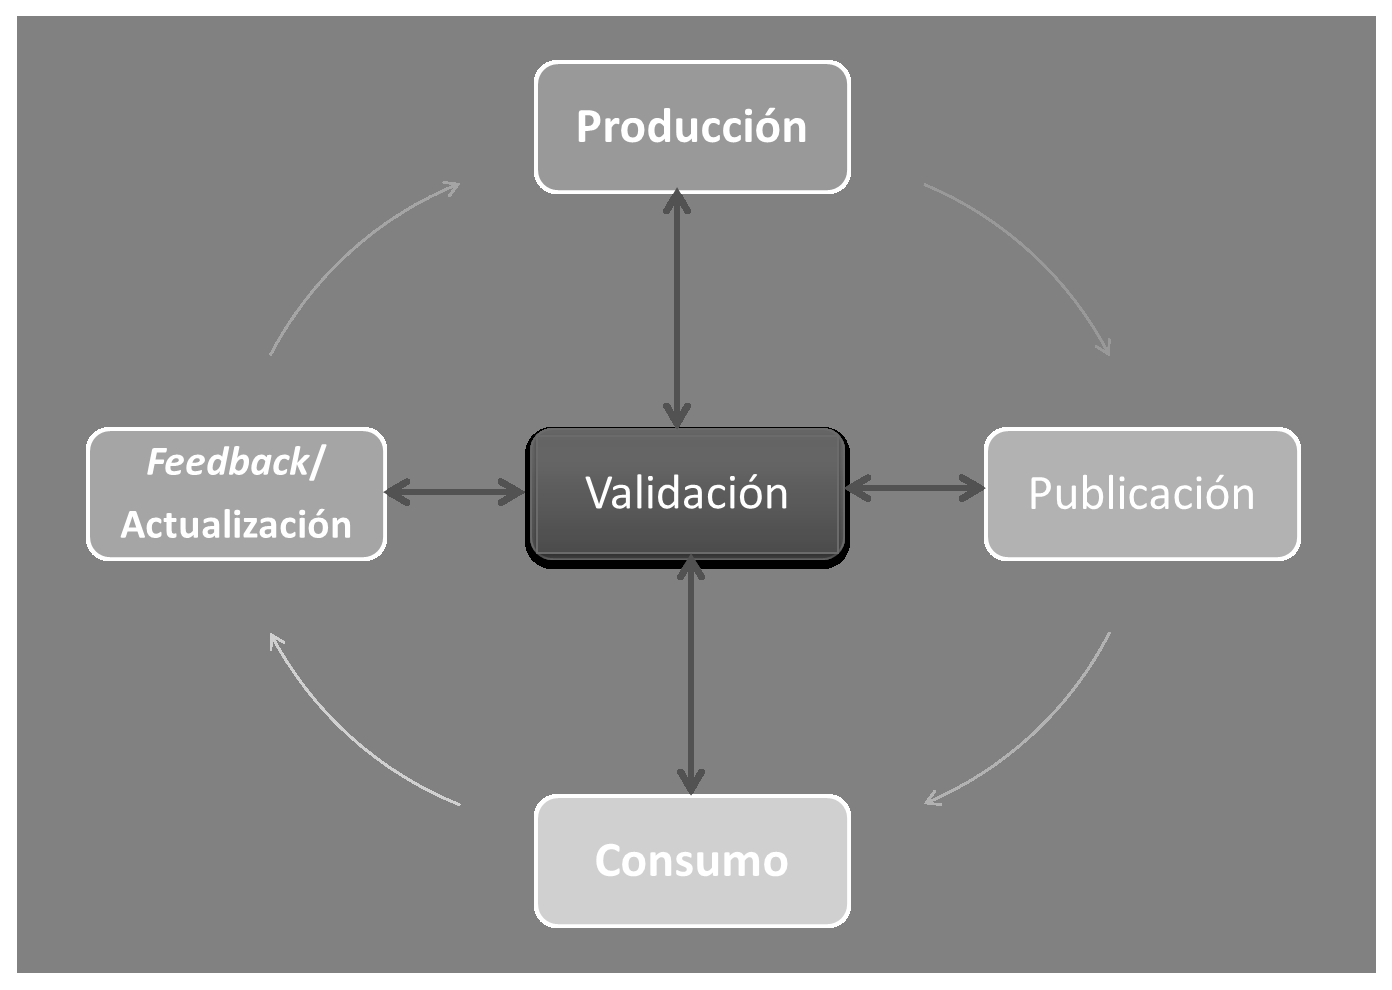
\includegraphics[width=16cm]{img/lld}
\caption{Procesos del Ciclo de Vida de Datos Enlazados Abiertos.}\label{lld}
\end{figure}

\begin{figure}[htb]
\centering
 \includegraphics[width=16cm]{img/ldl}
\caption{Flujo de tareas en el Ciclo de Vida de Datos Enlazados Abiertos.}\label{tareas}
\end{figure}

\section{Caso de Estudio: Las licitaciones públicas}
En el caso objeto de estudio de este documento se ha planteado la aplicación de los principios 
de \linkeddata, para el modelado y explotación de datos e información provenientes de los anuncios de 
licitación públicos. Para ello, tal y como se ha presentado en los anteriores apartados, se ha definido 
un ciclo de vida de datos enlazados que a través de procesos, métodos y tareas suministra una metodología 
de actuación genérica para proceder en este sentido. Como ejemplo de su validez y aplicación se han utilizado 
los datos de los contratos públicos para ejemplificar los procesos de producción, publicación, consumo, validación y 
actualización, ver Figura~\ref{fig:com}. Aunque ciertas tareas se apoyan en el uso de aplicaciones de terceros como Google Refine o bien 
en la parametrización de bibliotecas ya existentes como Apache Lucene, Mahout o Solr, es necesario suministrar un entorno 
en el cual los resultados de aplicación de las tareas puedan ser procesados para implementar algunas de las ya 
especificadas y así ejemplificar transversalmente el uso de datos enlazados en un determinado dominio. Por ello, y 
de acuerdo al análisis y especificación realizado se plantea la necesidad de diseñar los componentes del sistema 
MOLDEAS, ver Figuras~\ref{fig:com} y~\ref{moldeas}, como paso final para la cobertura en el uso de datos enlazados en el campo de la contratación pública 
electrónica y teniendo presentes los siguientes objetivos: 1) facilitar y dar soporte a las tareas del ciclo de vida que no puedan ser desarrolladas completamente 
por herramientas externas. 2)  Validar los datos generados por otras herramientas. 3) Enriquecer con procesos \textit{ad-hoc} la información y datos de los anuncios de licitación según el modelo 
y especificación fijado en el ciclo de vida. 4) Implementar un demostrador público de consumo de datos enlazados. 
5) Proveer un sistema de búsqueda/recomendación de anuncios de licitación de acuerdo a criterios predefinidos por el cliente. 6) Establecer un conjunto de prueba que realice la validación parcial de ciertos procesos apoyándose en tecnología 
pre-existente y 7) diseñar un sistema extensible y escalable para su futura ampliación.

\begin{figure}[htb]
\centering
 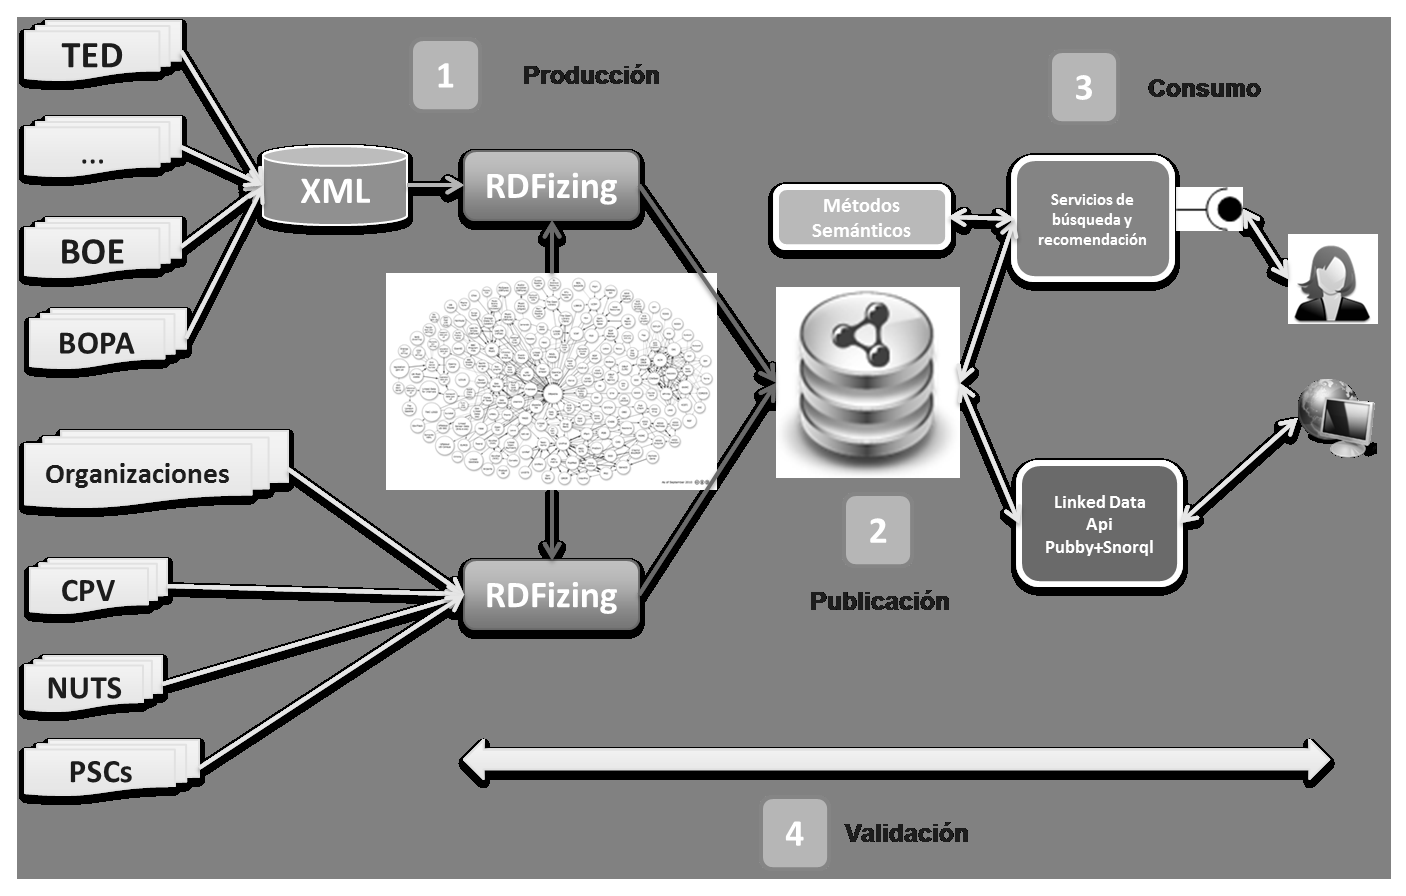
\includegraphics[width=14cm]{img/functional-overview}
\caption{Visión funcional de la plataforma MOLDEAS.}\label{moldeas}
\end{figure}


\begin{figure}[h]
\centering
\begin{tikzpicture}[scale=0.8, transform shape]
  \path[mindmap,concept color=gray,text=white]
    node[concept] {MOLDEAS}
    [clockwise from=0]
    child[concept color=green!50!black] {
      node[concept] {moldeas-api}   
      [clockwise from=-90]
      child [concept color=green!80] { node[concept] {\textbf{Consumo}} }   
    }  
    child[concept color=blue] {
      node[concept] {moldeas-transformer}
      [clockwise from=-90]
      child [concept color=blue!50] { node[concept] {\textbf{Producción}} }
      child [concept color=blue!50] { node[concept] {\textbf{Publicación}} }           
    }
    child[concept color=orange] { node[concept] {moldeas-test} 
      [clockwise from=-90]
      child  [concept color=orange!50] { node[concept] {\textbf{Validación}} }      
    }
    child[concept color=red] { node[concept] {moldeas-common} } ;
   
\end{tikzpicture}
    \caption{Alineación inicial de componentes de MOLDEAS y procesos del Ciclo de Vida de \linkeddata.}
 \label{fig:com}
\end{figure}

La aplicación del ciclo de vida de datos enlazados abiertos definido mediante la ejecución de los componentes 
del sistema MOLDEAS se ha realizado sobre la información de los anuncios de licitación que contienen tres grandes 
fuentes de información: 1) metainformación sobre el propio contrato, 2) clasificación del contrato de acuerdo a una 
clasificación estándar de productos (algunos ejemplos de estas clasificaciones son el ``Common Procurement Vocabulary''-CPV, ``Combined Nomenclature''-CN, 
FIXME) y 3) información geográfica y sobre las organizaciones o agentes implicados en el proceso. El resultado de esta transformación 
se puede ver en la Tabla~\ref{resultado} obteniendo un nuevo conjunto de datos enlazados enriquecido conteniendo cerca de 10 millones 
de tripletas RDF así como miles de enlaces a conjuntos de datos externos como los procedentes de NUTS, DBPedia o FAO. Esta transformación 
ha cubierto anuncios de licitación publicados en toda Europa (ej. TED) a nivel \textbf{nacional} (ej: ``Boletín Oficial de España''-BOE, 
\textbf{regional} (``Boletín Oficial del Principado de Asturias''-BOPA) y \textbf{local} (ej: ``Hospital Universitario Central de Asturias''). Una 
vez transformada esta información y datos se hace disponible al público siguiendo las directrices de \lod para su explotación tanto 
por usuarios finales como por máquinas, facilitando y potenciando su reutilización.

\begin{table}[!t]
  \centering
  \caption{Estadísticas de promoción de datos a la iniciativa \textit{Linked Open Data}.}\label{resultado}   
    \begin{tabular}{|p{2.5cm}|p{1.8cm}|p{3.5cm}|} 
    \hline
    \textbf{Tipo de Entidad} & \textbf{Nº de Elementos}  &  \textbf{Tripletas RDF}  \\\hline
     \multicolumn{3}{|c|}{\textbf{Catálogo de Anuncios de Licitación}} \\ \hline     
	PPN 2008 & $112843$  &   $677058$  \\ \hline
	PPN 2009 & $399766$ &   $2398601$   \\ \hline
	PPN 2010  & $431813$&  $2590880$  \\ \hline
        PPN 2011 & $67044$&   $402264$   \\ \hline
        \multicolumn{3}{|c|}{\textbf{Total}} \\ \hline
        PPNs & $1011466$ &  $6068803$   \\ \hline     
        \multicolumn{3}{|c|}{\textbf{Catálogo de Clasficaciones de Productos (PSCs)}} \\ \hline
        CPV 2003 & $8323$  & $546135$  \\ \hline
        CPV 2008 & $10357$ &  $803311$ \\ \hline
        CN 2012  & $14552$&  $137484$ \\ \hline
        CPC 2008 & $4408$&   $100819$\\ \hline
        CPA 2008 & $5429$&  $92749$ \\ \hline
        ISIC v4  & $766$&  $18986$  \\ \hline
        NAICS 2007 & $2328$&  $36292$   \\ \hline
      NAICS 2012 & $2212$&  $35390$    \\ \hline
      SITC v4 & $4017$&  $70887$    \\ \hline
      \multicolumn{3}{|c|}{\textbf{Total}} \\ \hline
      PSCs & $52392$ &   $1842053$  con $40351$ enlaces  \\ \hline
       \multicolumn{3}{|c|}{\textbf{Catálogo de organizaciones, personas y países}} \\ \hline
      Organizaciones & $50000$   & $1150020$   \\ \hline
      Personas & $50000$    & $900219$  \\ \hline
      Países y regiones & $246$     & $1756$  \\ \hline
           \multicolumn{3}{|c|}{\textbf{Total}} \\ \hline
       & $100246$  & $2051995$   \\ \hline
      \end{tabular}
 \end{table}   
 
Finalmente, la plataforma MOLDEAS~\footnote{\url{http://purl.org/weso/moldeas-web/}} mediante sus algoritmos de explotación de conocimiento es capaz de generar la consulta SPARQL 
motivadora, ver Figura~\ref{figure:expanded}, de esta trabajo (en la parte concerniente a explotación de datos) ajustando los parámetros de la consulta (por ejemplo 
la cuantía del contrato) al perfil definido por el usuario mediante el interfaz gráfico, ver Figura~\ref{fig:moldeas-web} .

\begin{figure}[!htb]
\centering
	\includegraphics[width=14cm]{./img/interfaz}
\caption{Interfaz de Usuario de la plataforma MOLDEAS.}
\label{fig:moldeas-web}
\end{figure}



 \begin{figure}[!ht] 
\begin{center}
\begin{lstlisting}[language=SPARQL]
SELECT * WHERE{
  ...
  ?notice nuts:containedBy ?place .
FILTER (  
  ( (?cpvCode =  cpv:45221000) 
  or (?cpvCode =  cpv:45221110) 
  or (?cpvCode =  cpv:45221111)...)
  ( (?place nuts:containedBy nuts:NL326) 
  or (?place nuts:containedBy nuts:B3) 
  or (?place nuts:containedBy nuts:BE2) 
  or ...) 
  and (?duration >= 2 and ?duration <= 4) 
  and (?date >= 2008 and ?date <= 2011) 
  and (?totalValue > 130,000^xsd:double 
  and ?totalValue <= 200,000^xsd:double))}
\end{lstlisting}
\caption{Consulta SPARQL generada por la plataforma MOLDEAS.}
\label{figure:expanded}
\end{center}
\end{figure}


\chapter{Experimentación}
Con el objetivo de validar el trabajo realizado mediante experimentos en los cuales se pueda cuantificar el 
enfoque realizado la experimentación posible es muy variada, pero atendiendo  a la hipótesis de partida y a 
los componentes implementados es posible identificar los siguientes experimentos: 1) experimento para la validación de los datos 
transformados desde un punto de vista cuantitativo y cualitativo; 2) experimento para la verificación de la construcción de 
un sistema de recuperación de información utilizando una fuente de datos basada en \linkeddata y tecnologías semánticas y 3) 
experimento para la evaluación del rendimiento del sistema construido desde un punto de vista cuantitativo.

El diseño de estos experimentos permite por una parte, la verificación de la hipótesis objeto de estudio en este trabajo y, por otra parte, 
la validación de la construcción de sistemas basados en \linkeddata y tecnologías semánticas. Es preciso señalar que todos los experimentos llevados a cabo se realizan 
bajo la ejecución de un plan detallado, las etapas a seguir han sido las siguientes:
\begin{enumerate}
 \item Definición de los objetivos del experimento. 
\item Selección de una regla de asignación de las unidades experimentales a las condiciones de estudio. 
\begin{itemize}
 \item Cualitativos: tipo de entorno hardware y software, etc. En este caso, se pueden fijar las condiciones \textit{hardware} y \textit{software}:
 \item Cuantitativos: tamaño de la muestra o de la memoria.
\end{itemize}
 \item Especificación de las medidas de trabajo en cuanto a la respuesta.
 \item Ejecución de un experimento piloto. 
 \item Especificación de un modelo.
 \item Esquematización de los pasos a seguir. 
 \item Determinación del tamaño muestral.
 \item Revisión de las decisiones anteriores.
\end{enumerate}

Los detalles pormenorizados de cada uno de los experimentos siguiendo estos pasos se pueden encontrar 
en el capítulo correpondiente en el documento de la tesis doctoral. A continuación, este trabajo 
se centrará en el objetivo y resultado de los experimentos.

\section{Experimento I}
El diseño de este experimento se planifica desde dos puntos de vista:
\begin{itemize}
 \item Cuantitativo. La pregunta principal planteada en este caso se refiere a la posibilidad del uso de datos enlazados para 
facilitar el acceso a un mayor número de recursos relacionados con los anuncios de licitación y, en consecuencia, a la información 
y datos disponibles en los mismos.
\item Cualitativo. La cuestión planteada en este caso se centra en valorar si el proceso de generación y transformación de datos 
a la iniciativa de datos enlazados se puede valorar respecto a una serie de criterios y buenas prácticas.
\end{itemize}

La ejecución del experimento \textit{cuantiativo} requiere la expresión formal de los datos, para establecer desde un punto 
de vista cuantitativo el porcentaje de ganancia en expresividad pasando de utilizar un vocabulario controlado para la realización 
de consultas, a una serie de los mismos mediante datos enlazados. En este caso, la recuperación de información 
entre la búsqueda habitual (texto libre) y un vocabulario controlado difiere en que el universo del discurso es, 
en el primer caso infinito y en el segundo finito, determinado por el número de términos del vocabulario. En los anuncios 
de licitación se parte de las siguientes premisas: 1) todo anuncio de licitación está etiquetado al menos 
con un código/término perteneciente al CPV 2008. 2) El uso de los códigos CPV es obligatorio en todos los anuncios de licitación a nivel europeo y 
3)la única información obligatoria, además del emisor del anuncio de licitación, son los códigos CPV 2008. Bajo estas circunstancias 
la muestra sobre la que se realiza el experimento cuenta con las siguientes características:
\begin{itemize}
 \item Se cuenta con una base documental $\mathcal{D}$ constituida por $1$ millón de anuncios de licitación.
 \item La clasificación de productos (vocabulario controlado $\mathcal{V}$ para contratos públicos) 
del CPV 2008 está formado $\#\mathcal{V} = 10357$ códigos/términos distintos.
 \item Cada uno de los documentos $d \in \mathcal{D}$ está etiquetado con al menos un código $v \in \mathcal{V}$.
\end{itemize}

Una vez caracterizado el entorno de pruebas, cabe formular cómo se calcula la ganancia de añadir un nuevo vocabulario 
mediante \linkeddata.
\begin{itemize}
 \item El nuevo vocabulario controlado $\mathcal{V}_{psc}$ dispone $\#\mathcal{V}_{psc}$ términos.
 \item El enlazado de datos que genera este vocabulario respecto a uno objetivo $\mathcal{V}$, presenta los siguientes
casos:
\begin{enumerate}
 \item Enlace 1-1, es decir, existen términos $v^k_{psc} \in \mathcal{V}_{psc}$ que se enlazan con un sólo término $v^k \in \mathcal{V}$ 
generando $K$ enlaces.
 \item Enlace 1-n, es decir, existen términos $v^k_{psc} \in \mathcal{V}_{psc}$ que se enlazan con varios términos $v^k \in \mathcal{V}$ 
generando $K_n$ enlaces.
\end{enumerate}
\item El resultado de esta operación es un conjunto de pares de enlaces $\{ (v^0_{psc},v^0), (v^k_{psc},v^k)..(v^n_{psc},v^n) \}$.
\item Dada esta situación, el vocabulario inicial $\mathcal{V}$ ha sido incrementado en todos los elementos $v^k_{psc} \in \mathcal{V}_{psc}$, 
para los cuales existe un enlace con algún elemento $v^k \in \mathcal{V}$ .
\item El número de nuevos términos en los que el vocabulario $\mathcal{V}$ es incrementado, es igual al conjunto 
de elementos $v^k_{psc}$, denominado  $\mathcal{V'}_{psc}$, con algún enlace a $\mathcal{V}$ (estrictamente sin repeticiones por definición de conjunto).
\item El porcentaje de ganancia de expresividad, en el sentido de cuántos nuevos términos permiten pasar de $\mathcal{V}_{psc}$ a 
$\mathcal{V}$, es el siguiente:

\begin{align}
\% =  \{ \langle (\#\mathcal{V'}_{psc}+\#\mathcal{V}) / \#\mathcal{V} \rangle - 1 \} * 100
\end{align}

\item Finalmente, y en el caso concreto de las clasificaciones de productos/taxonomías, existe la posibilidad de que elementos 
$v^j_{psc} \in \mathcal{V}_{psc}$ no estén directamente relacionados con el conjunto $\mathcal{V}$ pero de acuerdo a la jerarquía 
de términos en $\mathcal{V}_{psc}$ se puede deducir que si $v^j_{psc}$ está relacionado con $v^k_{psc}$ a través de una relación $r_k$, 
entonces $v^j_{psc} \in \mathcal{V'}_{psc}$. Este tipo de enfoque es crítico debido a que provoca una situación recursiva e infinita, 
uno de los problemas actuales de \linkeddata en la ejecución de consultas, pero debido a que el vocabulario $\mathcal{V}_{psc}$ es 
finito y las relaciones entre sus términos es de jerarquía, se puede establecer un valor máximo para el porcentaje de 
ganancia que ocurrirá cuando $\mathcal{V}_{psc} \equiv \mathcal{V'}_{psc}$.

\end{itemize}

Adicionalmente e introduciendo un nivel más de indirección mediante las PSCs con \textit{ProductOntology-PO} surge el siguiente caso:
\begin{itemize}
 \item Existe un conjunto $\mathcal{V''}_{psc}$ que representa la unión de todos los $\mathcal{V'}_{psc}$ correspondientes 
a los enlaces entre una determinada PSC y \textit{PO}, estrictamente conteniendo el elemento de \textit{PO} de cada par.
\item Existe un conjunto $\mathcal{V'}_{cpv}$ que representa el conjunto de pares de enlaces entre el CPV 2008 y \textit{PO}, 
estrictamente conteniendo el elemento de \textit{PO} de cada par.
\item La intersección entre $\mathcal{V''}_{psc} \sqcap \mathcal{V'}_{cpv}$ representa el conjunto de todos enlaces mediante 
los cuales se puede realizar el salto entre una PSC al CPV 2008 a través de \textit{PO}. Los elementos 
de cada PSC que permitan acceder al CPV 2008 de esta forma y no se encuentren en el conjunto $\mathcal{V'}_{psc}$ de cada PSC, señalado 
en la Tabla~\ref{ganancia-terminos}, deben ser también considerados como nuevos términos para la realización de consultas generando 
un nuevo conjunto $\mathcal{V''}_{psc}$.
\end{itemize}

De acuerdo a estas definiciones, en la Tabla~\ref{ganancia-terminos} y en la Figura~\ref{fig:eval-n-terminos} 
se presentan los porcentajes reales y máximos obtenidos tras la realización del enlazado de las clasificaciones 
de productos con el CPV 2008, conjunto $\mathcal{V}$ con $\#\mathcal{V} = 10357$. Bajo estas condiciones, 
el paradigma basado en \linkeddata permite que, a través de una correcta aplicación de un ciclo de vida para la generación 
de las clasificaciones de productos en RDF y su enlazado posterior, se suministre el soporte necesario para cumplir con 
las premisas fijadas aumentando la capacidad expresiva del vocabulario de entrada (de $10357$ a $21715$ y con 
un máximo de $39586$ a través de \textit{PO}) y para la recuperación de información de los anuncios de licitación pública, 
aumentando así la capacidad expresiva para la realización de consultas o extracción de estadísticas. 

\begin{table}[!t]
  \centering
  \caption{Porcentaje de Ganancia Real y Máxima al enlazar las Clasificaciones de Productos con el CPV 2008.}\label{ganancia-terminos}   
%
    \begin{tabular}{|p{2.6cm}|p{1.8cm}|p{1.8cm}|p{1.8cm}|p{1.8cm}|p{1.8cm}|p{1.8cm}|} 
     \hline
    $\mathcal{V}_{psc}$ & $\#\mathcal{V}_{psc}$  & $\#\mathcal{V'}_{psc}$ &$\#\mathcal{V'''}_{psc}$ &  $\%$ real &  $\%$ real con PO  &  $\%$ máximo   \\\hline
    CPV 2003 	& $8323$  	& $462$		& $8312$ 	& $4.46$ 	& $80.25$	& $80.36$  \\ \hline
    CN 2012  	& $14552$	& $2390$	& $2390$ 	& $23.07$	& $23.07$	& $140.50$  \\ \hline
    CPC 2008 	& $4408$	& $4402$   	& $4403$	& $42.50$	& $42.51$ 	& $42.56$  \\ \hline
    CPA 2008 	& $5429$	& $5399$   	& $5410$	& $52.12$	& $52.23$	& $52.41$  \\ \hline
    ISIC v4  	& $766$		& $765$   	& $765$ 	& $7.38$ 	& $7.38$	& $7.39$    \\ \hline
    NAICS 2007 	& $2328$	& $2300$ 	& $2300$	& $22.20$	& $22.20$	& $22.47$  \\ \hline
    NAICS 2012 	& $2212$	& $2186$ 	& $2186$	& $21.10$	& $21.10$	& $21.35$  \\ \hline
    SITC v4 	& $4017$	& $3811$   	& $3820$	& $36.79$	& $36.88$	& $38.78$  \\ \hline
    \multicolumn{7}{|c|}{\textbf{Total}} \\ \hline
    $\star$ & $42035$ 		& $21715$   	& $29586$	& $209.66$ 	& $285.66$	& $405.86$ \\ \hline
    \hline
    \multicolumn{7}{|c|}{\textbf{Añadiendo enlaces entre CPV 2008 y \textit{Product Ontology}}} \\ \hline
    \textit{PO}& $\infty$	& $10000$   	& N/A	& $96.55$	& $96.55$ 	& $\infty$  \\ \hline
    \multicolumn{7}{|c|}{\textbf{Total con vocabulario de \textit{Product Ontology}}} \\ \hline
    $\star$	 & $\infty$	& $31715$   	& $39586$	& $306.21$	& $382.21$	& $\infty$ \\ \hline
    \hline
  \end{tabular}

\end{table}

\begin{figure}[!htb]
\centering
  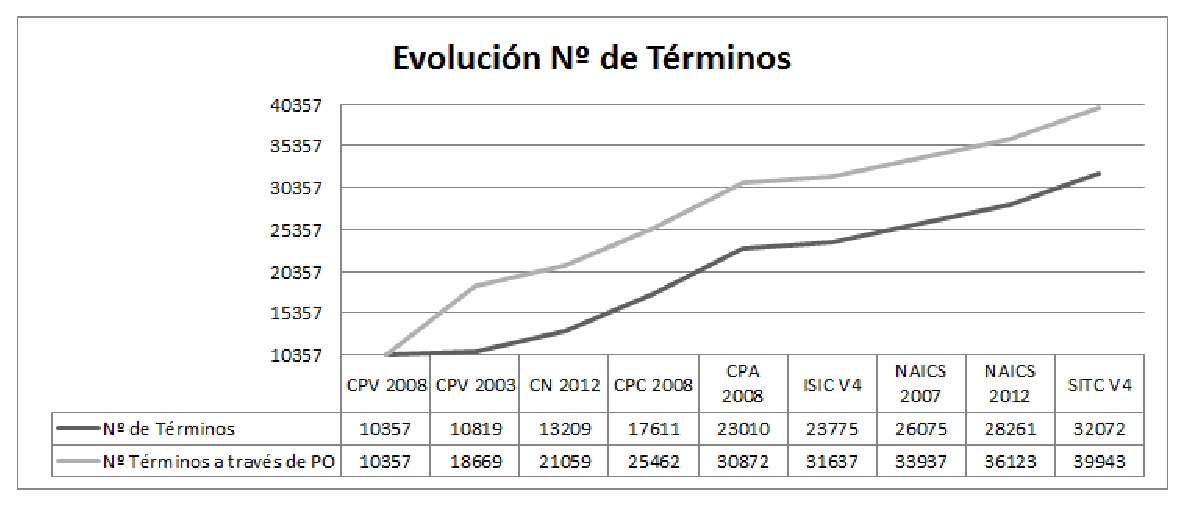
\includegraphics[width=12cm]{./img/evo-n-terminos}
\caption{Evolución Número de Términos.}
\label{fig:eval-n-terminos}
\end{figure}



El experimento y evaluación \textbf{cualitativa} realizada permiten realizar una calificación y comparación entre los distintos enfoques 
disponibles para la publicación y acceso a la información y datos referente a los anuncios de licitación, incluyendo
el catálogo de clasificaciones de productos y las organizaciones. Para ello, se han definido una serie de tablas 
con una serie de características en el ámbito de \linkeddata, \opendata y \lod que sirvan para verificar que
la aplicación de los métodos semánticos es correcta y con ello obtener datos enlazados que aporten las ventajas conocidas sobre el uso
de esta iniciativa. La elaboración de estas tablas, cubriendo un total de 196 criterios, surge de la agregación de varias fuentes: 1) Principios de \linkeddata~\cite{Berners-Lee-2006}. 2) Principios de \opendata~\cite{okfn}. 
3) Especificaciones y documentos del W3C como~\cite{publishing-ogd,linked-data-cookbook,Berr08}. 4) \textit{Linked Data Design Considerations}~\cite{Heath_Bizer_2011}. 5) \textit{Linked Data Patterns}~\cite{linked-data-patterns}. 
5)``\textit{Basic Profile Resources}''~\cite{basic-profile-ibm} de IBM. 6) Principios para incluir \datasets en la nube de datos 
enlazados y añadir al registro de CKAN y 7) Documentación específica de iniciativas nacionales y experiencia adquirida. El 
modelado de estas tablas es la de un cuestionario, de manera que la evaluación de una característica puede tener las siguientes 
respuestas: 1) Positiva \si. La característica es aplicable y se ha realizado en el actual \dataset. 2) 
Negativa \no. La característica es aplicable y no se ha realizado en el actual \dataset y 3) No aplicable \na. 
La característica no es aplicable y no se ha realizado en el actual \dataset. Los resultados agregados se pueden observar en la 
Tabla~\ref{tabla:agregado-sumatorio}, la tendencia que se observa  es que la información y datos relativa a los anuncios de licitación, 
clasificaciones de productos y organizaciones tiene un carácter abierto, como confirman los resultados, e incluso disponen
de buenos fundamentos para que la realización del esfuerzo de transformación a datos enlazados sea asumible tanto 
por las Administraciones Públicas como por terceros, así lo demuestra el trabajo presentado en este documento 
a través del enfoque realizado en MOLDEAS. La aplicación de los principios de \linkeddata y \opendata permite 
asegurar ventajas y beneficios en el acceso a la información y manejo de los datos.

\begin{table}[!t]
  \centering
  \caption{Tabla agregada de Validación Conjunta con Valores Totales.}\label{tabla:agregado-sumatorio}
      \begin{tabular}{|p{4cm}|p{1.5cm}|p{1.5cm}|p{1.5cm}||p{2cm}||p{2cm}|} 
           \hline
       \textbf{Versión} & \si&\no&\na & \textbf{Total} & \textbf{\% \si entre aplicables} \\\hline
          \textbf{Referencia} & 173 & 0 & 23 & 196& 100 \\ \hline \hline
	\multicolumn{6}{|c|}{\textbf{Anuncios de Licitación}} \\ \hline   
	    \textbf{TED} & 32 & 12 & 152 &$\equiv$ & $72.72$\\ \hline 
	    \textbf{Plataforma de Contratación} & 35 & 9 & 152 &$\equiv$ & $79.54$\\ \hline 
	    \textbf{BOE} & 30 & 12 & 154 &$\equiv$ & $71.42$\\ \hline 
	    \textbf{Servicios Externos} & 25 & 14 & 157 &$\equiv$ & $64.10$\\ \hline 
	    \textbf{LOTED} & 92 & 34 & 70 &$\equiv$ & $73.01$\\ \hline 
	    \textbf{MOLDEAS} & 121 & 10 & 65 &$\equiv$ & $92.36$\\ \hline 
	\multicolumn{6}{|c|}{\textbf{Catálogo de Clasificaciones de Productos}} \\ \hline
	    \textbf{CSV/MSExcel} &  25 & 12 & 159 &$\equiv$ & $67.56$\\ \hline 
	    \textbf{Servicios on-line} &  21 & 21 & 154 &$\equiv$ & $50$\\ \hline 
	    \textbf{MOLDEAS} &  166 & 7 & 23 &$\equiv$ & $93.86$\\ \hline 
	\multicolumn{6}{|c|}{\textbf{Organizaciones}} \\ \hline
	    \textbf{TED} & 20 & 9 & 167 &$\equiv$ & $68.96$\\ \hline 
	    \textbf{Plataforma de Contratación}  & 35 & 10 & 151 &$\equiv$ & $77.77$ \\ \hline 
	    \textbf{BORME}  & 23 & 1 & 172 &$\equiv$ & $95.83$\\ \hline 
	    \textbf{Servicios Externos}  & 20 & 20 & 156 &$\equiv$ & $50$\\ \hline   
	    \textbf{BBDD externa}  & 12 & 9 & 175 &$\equiv$ & $57.14$\\ \hline 
	    \textbf{OpenCorporates}  & 85 & 33 & 78  &$\equiv$ & $72.03$\\ \hline 
	    \textbf{MOLDEAS}  & 121 & 10 & 65 &$\equiv$ & $92.36$\\ \hline 
          \end{tabular}
 \end{table} 
 
\section{Experimento II}
La especificación del experimento sobre la recuperación de información en anuncios de licitación se ha abordado 
con los dos grandes objetivos de consumir los datos enlazados producidos e implementar un demostrador público que permita realizar 
búsquedas avanzadas y contextuales sobre la información disponible.  En este caso y centrándose en el 
tamaño de la muestra se han obtenido las consultas presentadas en la Tabla~\ref{table:queries-ir}, de las 
cuales se tiene la siguiente información: consulta proporcionada por un cliente, $Q_{str}$, y códigos CPV seleccionados por los expertos 
de dominio de ``Euroalert.net'', $Q_{cpv}$. Debido al gran número de códigos CPV tan sólo se muestra la cantidad de los mismos esquivando 
el código y la descripción.  Sintetizando, el experimento que se realiza, evalúa los códigos CPV generados (o recuperados) mediante el sistema MOLDEAS, 
ver Tabla~\ref{table:metodos-ir}, en contraposición con los suministrados por ``10ders Information Services'' y utilizando las medidas de evaluación Precisión (P), \textit{Recall} (R), \textit{Accuracy} (A) y 
\textit{Especificidad} (S). 

Según los resultados obtenidos, ver Tabla~\ref{table:queries-ir-results}, y de acuerdo al comportamiento de los expertos del dominio, queda patente que el 
método $M^1$ es el más cercano a los resultados esperados. La explicación se debe principalmente al grado de implantación que 
posee la búsqueda tradicional. No obstante, tan sólo se han utilizado $11$ consultas \linebreak preparadas (no se disponía de una muestra mayor) 
por lo que los resultados bajo estas condiciones y sin un contraste de hipótesis estadístico, deben ser tomados como una guía, en la cual la valoración con una muestra 
de la población relevante e informativa podrían variar. Este experimento sirve como prueba del consumo de datos enlazados en un 
dominio y de la aplicación de técnicas tanto tradicionales como procedentes de otros ámbitos para la recuperación de códigos CPV. 
La principal conclusión que se debe extraer, consiste en que el planteamiento de un sistema experto para la recuperación de anuncios de licitación 
públicos tiene un gran interés debido a diversos factores: variables de información múltiples, correlaciones entre las mismas, 
cantidad de datos a procesar, etc., que pueden ser optimizados a través de las pruebas con distintos algoritmos y técnicas.

\begin{table}[!t]
  \centering
\caption{Métodos de generación de códigos CPV.}\label{table:metodos-ir}   
\begin{tabular}[!t]{|l|p{6cm}|p{4cm}|} 
\hline  
\textbf{Método} &  \textbf{Descripción} &  \textbf{Tecnología} \\\hline
$M^1$ & Indexa códigos CPV y búsqueda sintáctica. & Apache Lucene y Solr \\ \hline
$M^2$ & Extrae códigos CPV candidatos ponderados, atendiendo a las relaciones semánticas. & $M^1$ + ponderación jerarquía \\ \hline
$M^3$ & Extrae códigos CPV candidatos ponderados mediante \textit{Spreading Activation}. & $M^1$ + ONTOSPREAD \\ \hline
$M^4$ & Extrae códigos CPV candidatos ponderados según el histórico del $1$ M con un motor de recomendación. & $M^1$ + Apache Mahout \\ \hline
\hline
 \end{tabular}
   \end{table} 


\begin{table}[!t]
  \centering
  \caption{Consultas suministradas en el proyecto ``10ders Information Services''.}\label{table:queries-ir}    
\begin{tabular}[c]{|l|p{10cm}|p{3cm}|} 
\hline
\textbf{$Q_{i}$} &  \textbf{Consulta de Usuario-$Q_{str}$} &  \textbf{Nº de Códigos CPV relevantes-$\#Q^{i}_{cpv}$} \\\hline
$Q_1$ & ``Comprehensive overview over all environmental technologies renewable energy products'' & $463$ \\ \hline
$Q_2$ & ``Tendering of public works: housing, hospitals, roads, housing developments, station drinking water treatment, reforestation'' & $35$ \\ \hline
$Q_3$ & ``Prefabricated buildings'' & $7$ \\ \hline
$Q_4$ & ``Games for children (parks swings, slides, land of play equipment in the public sphere'' & $26$ \\ \hline
$Q_5$ & ``Vital signs monitor'' &  $277$\\ \hline
$Q_6$ & ``Museum and exhibition and product launch services'' & $1$ \\ \hline
$Q_7$ & ``Voltmeters, instruments measuring electrical quantities, Ammeters, Instruments for checking physical characteristics, hygrometers, thermometers, measuring equipment and control, leak detector, Analyzers, 
Cable Splicing insulated cable joints kits, screwdrivers, hand tools , screwdriver'' & $117$ \\ \hline
$Q_8$ & ``Conservation Maintenance of pavements for roads, airfields, bridges, tunnels'' & $13$ \\ \hline
$Q_9$ & ``Wood poles, Wooden sleepers , Lattice towers'' & $10$ \\ \hline
$Q_{10}$ & ``Architectural, construction, engineering and inspection services'' &  $173$\\ \hline
$Q_{11}$ & ``Medical practice and related services'' &  $13$\\ \hline
\hline
 \end{tabular}

 \end{table} 


\begin{sidewaystable}[!t]
  \centering
  \caption{Resultados PRAS de las consultas suministradas en el proyecto ``10ders Information Services''.}\label{table:queries-ir-results}
\begin{tabular}{|c||c|c|c|c||c|c|c|c||c|c|c|c||c|c|c|c|}
\hline
 \textbf{$Q_i$}&\multicolumn{4}{|c||}{$M^{1}$} & \multicolumn{4}{|c||}{$M^{2}$}& \multicolumn{4}{|c||}{$M^{3}$} & \multicolumn{4}{|c|}{$M^{4}$} \\ \hline
	  &\textbf{P} & \textbf{R} & \textbf{A} & \textbf{S} &		\textbf{P} & \textbf{R} & \textbf{A} & \textbf{S} &			\textbf{P} & \textbf{R} & \textbf{A} & \textbf{S} &		\textbf{P} & \textbf{R} & \textbf{A} & \textbf{S}  \\ \hline \hline
$Q_1$  	  &$0,15$ & $0,08$ & $0,94$ & $0,98$ &		$0,15$ & $0,15$ & $0,92$ & $0,96$ &	$0,12$ & $0,06$ & $0,94$ & $0,98$ &	$0,06$ & $0,06$ & $0,68$ & $0,81$ \\ \hline
$Q_2$  	  &$0,09$ & $0,09$ & $0,99$ & $1,00$ & 		$0,06$ & $0,06$ & $0,99$ & $1,00$ & 	$0,03$ & $0,03$ & $0,99$ & $1,00$ & 	$0,03$ & $0,03$ & $0,99$ & $1,00$ \\ \hline
$Q_3$  	  &$0,14$ & $0,14$ & $1,00$ & $1,00$ & 		$0,14$ & $0,14$ & $1,00$ & $1,00$ & 	$0,14$ & $0,14$ & $1,00$ & $1,00$ & 	$0,00$ & $0,00$ & $1,00$ & $1,00$ \\ \hline
$Q_4$  	  &$0,19$ & $0,19$ & $1,00$ & $1,00$ &		$0,00$ & $0,00$ & $0,99$ & $1,00$ & 	$0,12$ & $0,12$ & $1,00$ & $1,00$ & 	$0,00$ & $0,00$ & $0,99$ & $1,00$ \\ \hline
$Q_5$  	  &$0,12$ & $0,01$ & $0,97$ & $1,00$ & 		$0,01$ & $0,01$ & $0,95$ & $0,97$ & 	$0,08$ & $0,01$ & $0,97$ & $1,00$ & 	$0,03$ & $0,03$ & $0,95$ & $0,97$ \\ \hline
$Q_6$  	  &$1,00$ & $1,00$ & $1,00$ & $1,00$ & 		$0,00$ & $0,00$ & $1,00$ & $1,00$ & 	$1,00$ & $1,00$ & $1,00$ & $1,00$ & 	$0,10$ & $0,67$ & $0,98$ & $0,98$ \\ \hline
$Q_7$  	  &$0,20$ & $0,20$ & $0,98$ & $0,99$ & 		$0,09$ & $0,09$ & $0,98$ & $0,99$ & 	$0,15$ & $0,16$ & $0,98$ & $0,99$ & 	$0,03$ & $0,03$ & $0,98$ & $0,99$ \\ \hline
$Q_8$  	  &$0,08$ & $0,08$ & $1,00$ & $1,00$ & 		$0,08$ & $0,08$ & $1,00$ & $1,00$ & 	$0,08$ & $0,08$ & $1,00$ & $1,00$ & 	$0,00$ & $0,00$ & $1,00$ & $1,00$ \\ \hline
$Q_9$  	  &$0,50$ & $0,50$ & $1,00$ & $1,00$ & 		$0,00$ & $0,00$ & $1,00$ & $1,00$ & 	$0,30$ & $0,38$ & $1,00$ & $1,00$ & 	$0,00$ & $0,00$ & $1,00$ & $1,00$ \\ \hline
$Q_{10}$  &$0,39$ & $0,39$ & $0,98$ & $0,99$ & 		$0,42$ & $0,42$ & $0,98$ & $0,99$ & 	$0,34$ & $0,35$ & $0,98$ & $0,99$ & 	$0,16$ & $0,16$ & $0,97$ & $0,99$ \\ \hline
$Q_{11}$  &$0,23$ & $0,23$ & $1,00$ & $1,00$ & 		$0,23$ & $0,23$ & $1,00$ & $1,00$ & 	$0,15$ & $0,17$ & $1,00$ & $1,00$ & 	$0,00$ & $0,00$ & $1,00$ & $1,00$ \\ \hline
\multicolumn{17}{|c|}{\textbf{Medias Totales de Métricas PRAS}} \\ \hline
\textbf{Total}  &$0,28$ & $0,26$ & $0,99$ & $1,00$ & 	$0,11$ & $0,11$ & $0,98$ & $0,99$ & 	$0,23$ & $0,23$ & $0,99$ & $1,00$ & 	$0,03$ & $0,03$ & $0,96$ & $0,98$ \\ \hline
\hline
 \end{tabular}

 \end{sidewaystable} 
  
\section{Experimento III}
El objetivo de un experimento es averiguar si unos determinados factores influyen en una determinada variable de interés para así poder cuantificar dicha influencia. En el caso 
de esta sección, la variable a estudiar es el rendimiento de las consultas \gls{SPARQL} contra el \textit{endpoint} utilizado, si bien 
no es el experimento principal de este documento ya que conllevaría la comparación con distintos proveedores de 
repositorios \gls{RDF}, si que ha surgido la necesidad de abordar esta cuestión por la latencia en las consultas. La metodología utilizada 
para el diseño del experimento es la repetición, en condiciones indistinguibles, con el objetivo de minimizar la variabilidad 
del mismo y que el error experimental sea lo más pequeño posible.

\begin{table}[!ht]
\renewcommand{\arraystretch}{1.3}
\begin{center}
\begin{tabular}{|p{3cm}|p{2.5cm}|p{3.5cm}|p{3.5cm}|}
\hline
  \textbf{ID Consulta} & \textbf{Código CPV inicial} & \textbf{Códigos CPV expandidos} & \textbf{Códigos NUTS}  \\ \hline
  $Q_1$ & 15331137 & 48611000, 48611000, 50531510, 15871210 & UK, PL, RO \\ \hline
  $Q_2$ & 50531510 & 34144100, 44212211, 44212212, 50531500 & ES, FR, DE \\ \hline
  $Q_3$ & 34144100 & 44212211, 31140000, 31140000, 34144100 & PL, CZ, RO \\ \hline
  $Q_4$ & 64122000 & 64216120, 79571000, 15871210, 64121000 & BE, SE, DE \\ \hline
  $Q_5$ & 79320000 & 75241000, 75100000, 75000000, 60112000 & UK, FR, AT \\ \hline
  $Q_6$ & 44100000 & 44110000, 44170000, 44190000, UB03 & NL, SE, DE \\ \hline
  $Q_7$ & 31000000 & 33141000, 39000000, 44000000, 31600000 & DE, IT, HU \\ \hline
  $Q_8$ & 50000000 & 50512000, 50333100, 50530000, 50532300 & UK, IR, FR \\ \hline
  $Q_9$ (random)   & 15841400 & 15841300, 15511700, 44921210, 03131400 & ES, FR, DK \\ \hline
  \hline
  \end{tabular}
  \caption{Descripción de los códigos en las consultas en SPARQL del experimento.}
  \label{tabla:queries}
  \end{center}
\end{table} 


En referencia a los aspectos cuantitativos del experimento, el tamaño de la muestra consta de nueve consultas ($Q_{1..9}$), el número de réplicas 
para evitar el ruido y la aleatoriedad previamente comentada es de $3$ y la situación de partida para cada una de ellas se produce 
bajo las mismas condiciones: reinicio de la máquina y consultas de entrenamiento (1 simple y 1 expandida) antes de la ejecución de una réplica para la obtención 
de las observaciones de tiempo de ejecución. Referente al tamaño de la muestra, se utilizará el \textit{endpoint} descrito anteriormente y con la carga 
de tripletas generada a partir de la aplicación de los métodos semánticos a los anuncios de licitación y siguiendo la distribución por 
grafos nombrados especificada en el Sección~\ref{sect:pscs-data-model}.

Por otra parte, las características, $F_i$, a evaluar en combinación se presentan en la siguiente Tabla~\ref{table:sparql-features}, en resumen se parte de una 
consulta simple (1 código CPV y 1 código NUTS) para obtener un tiempo de referencia, a partir de esta primera referencia se aplican 
las distintas optimizaciones, generando los distintos tratamientos ($T_i$), ver Tabla~\ref{tabla:tests}, para el establecimiento de la mejor combinación posible.
\begin{enumerate}
  \item Especificación de las medidas de trabajo en cuanto a la respuesta. El valor que se toma es el tiempo de ejecución 
en segundos de la consulta en SPARQL. 
 \item Ejecución de un experimento piloto. Evidentemente esta tarea se ha realizado con una pequeña muestra de consultas, sólo un año de anuncios 
de licitación pero ejecutando todos los tratamientos con el fin de validar el enfoque propuesto, obtener los resultados de toma de tiempos y preparar 
el procesamiento del registro de tiempos para obtener las medidas finales.
 \item Especificación de un modelo. En este caso, no se utilizará un modelo matemático para aproximar los valores, 
como ya se ha explicado anteriormente, debido a que el objetivo es optimizar la realización de consultas, en cuanto a 
tiempo de ejecución, no a la predicción futura.
 \item Esquematización de los pasos a seguir.
 \item Determinación del tamaño muestral. Como ya se ha comentado anteriormente, en el apartado de factores cuantitativos, se utilizarán los datos generados durante el proceso de promoción 
de datos a \linkeddata de los anuncios de licitación y de las clasificaciones de productos.
 \item Revisión de las decisiones anteriores.
\end{enumerate}

\newpage
\begin{longtable}[c]{|l|p{10cm}|} 
\hline
\textbf{ID} &  \textbf{Descripción}  \\\hline
\endhead
$F_1$ & Consulta simple: $1$ código CPV y $1$ código NUTS \\ \hline
$F_2$ & $F_1$ con uso de la claúsula \texttt{LIMIT} de SPARQL \\ \hline
$F_3$ & Consulta expandida: $n$ códigos CPV y $n$ código NUTS  \\ \hline
$F_4$ & Reescritura de las consultas SPARQL: \texttt{FILTER}, etc.  \\ \hline
$F_5$ & Uso de grafos nombrados en la consulta SPARQL: claúsula \texttt{FROM} \\ \hline
$F_6$ & Separación de las consultas en SPARQL en simples ($F_1$) \\ \hline
$F_7$ & Consultas simples distribuidas con $5$ hilos (1 por código CPV) \\ \hline
\hline
\caption{Características de las consultas en SPARQL.}\label{table:sparql-features}\\    
\end{longtable}


\begin{table}[!htb]
\renewcommand{\arraystretch}{1.3}
\begin{center}
\begin{tabular}{|p{3.5cm}|p{0.8cm}|p{0.8cm}|p{0.8cm}|p{0.8cm}|p{0.8cm}|p{0.8cm}|p{0.8cm}|p{2cm}|}
\hline
  \textbf{Test}/ \textbf{Característica}& \textbf{$F_1$} & \textbf{$F_2$} & \textbf{$F_3$} & \textbf{$F_4$} & \textbf{$F_5$} & \textbf{$F_6$} &  \textbf{$F_7$} & \textbf{Nº consultas SPARQL} \\ \hline
   $T_1$ & $\star$ & & & & & & &$1$\\ \hline 
   $T_2$ & $\star$ & & $\star$ & & & & &$1$\\ \hline 
   $T_3$ &  & $\star$ &  & & & & &$1$\\ \hline 
   $T_4$ &  & $\star$ & $\star$ & & & & &$1$\\ \hline 
   $T_5$ &  & $\star$ & $\star$ & $\star$ & & & &$1$\\ \hline 
   $T^{1}_6$ ($n$ códigos CPV y $m$ códigos NUTS)&  & $\star$ & $\star$ & $\star$ & $\star$ & $\star$ & &$4$\\ \hline 
   $T^{2}_6$ ($\equiv$)&  & $\star$ & $\star$ & $\star$ & $\star$ & $\star$ & $\star$ &$4$\\ \hline 
   $T^{1}_7$ ($1$ código CPV y $m$ códigos NUTS) &  & $\star$ & $\star$ & $\star$ &  & $\star$ &  &$5$ \\ \hline 
   $T^{2}_7$ ($\equiv$) & & $\star$ & $\star$ & $\star$ &  & $\star$ & $\star$ &$5$\\ \hline 
   $T^{1}_8$ ($\equiv$)& & $\star$ & $\star$ & $\star$ & $\star$ & $\star$ &  &$20$\\ \hline 
   $T^{2}_8$ ($\equiv$) & & $\star$ & $\star$ & $\star$ & $\star$ & $\star$ &  $\star$ &$20$\\ \hline 
   $T^{1}_9$ ($1$ código CPV y $1$ código NUTS ) & & $\star$ & $\star$ & $\star$ &  & $\star$ & &$15$  \\ \hline 
   $T^{2}_9$ ($\equiv$)& & $\star$ & $\star$ & $\star$ & & $\star$ &  $\star$ &$15$\\ \hline 
   $T^{1}_{10}$ ($\equiv$) & & $\star$ & $\star$ & $\star$ & $\star$ & $\star$ & &$60$  \\ \hline 
   $T^{2}_{10}$ ($\equiv$) & & $\star$ & $\star$ & $\star$ & $\star$ & $\star$ & $\star$ &$60$ \\ \hline 
  \hline
  \end{tabular}
  \caption{Descripción de cada uno de los tratamientos, características de optimización.}
  \label{tabla:tests}
  \end{center}
\end{table} 

La aplicación del plan previsto en la anterior sección arroja un conjunto de valores para cada uno de los tratamientos ($T_k$) y réplicas de los tiempos 
de ejecución de las consultas, de acuerdo a las distintas características ($F_i$). En la Tabla~\ref{tabla:tests-agregado} se reflejan 
las medias de tiempo y ganancia agregadas de cada uno de los tratamientos realizados. Por otra parte, se presentan igualmente 
las medidas pormenorizadas de las observaciones realizadas y agregadas de las 3 réplicas ejecutadas, ver Tablas~\ref{tabla:results-1} y~\ref{tabla:results-2}. 
El cálculo de la ganancia se realiza mediante la fórmula: $t_{old}/t_{new}-1*100$, tomando como referencia para $T_2$, el tiempo de $T_1$ y para 
los tratamientos $T_{4..10}$, el tiempo de $T_3$. Finalmente, la ejecución de todos los tratamientos con las distintas observaciones y 
réplicas ha implicado la realización de $5751$ consultas en SPARQL, más las de entrenamiento para cada una de las réplicas. 

\begin{table}[!htb]
\renewcommand{\arraystretch}{1.3}
\begin{center}
\begin{tabular}{|l|c|c|}
\hline
  \textbf{Test}& \textbf{$\bar{X}$ Tiempo (seg.)} & \textbf{$\bar{X}$ Ganancia (\%)} \\ \hline
   $T_1$ & $3.21$  & N/A\\ \hline 
   $T_2$ & $3.25$  & $1.21$   \\ \hline 
   $T_3$ & $20.548$ & N/A   \\ \hline 
   $T_4$ & $20.552$ & $-0.02$ \\ \hline 
   $T_5$ & $20.545$ & $-0.01$ \\ \hline 
   $T^{1}_6$ & $20.52$  & $0.14$\\ \hline 
   $T^{2}_6$ & $11.80$ & $74.37$\\ \hline 
   $T^{1}_7$ & $15.81$ & $30.58$ \\ \hline 
   \textbf{$T^{2}_7$} & \textbf{$10.51$} & \textbf{$96.54$} \\ \hline
   $T^{1}_8$ & $32.33$ & $-36.11$ \\ \hline 
   $T^{2}_8$ & $18.45$ & $11.21$ \\ \hline 
   $T^{1}_9$ & $22.53$ & $-8.77$ \\ \hline 
   $T^{2}_9$ & $12.61$ & $63.36$ \\ \hline 
   \textbf{$T^{1}_{10}$} & \textbf{$71.01$} & $-70.97$ \\ \hline 
   $T^{2}_{10}$ & $35.08$ & $-40.42$ \\ \hline 
  \hline
  \end{tabular}
  \caption{Tiempo de ejecución (seg.) y ganancia (\%).}
  \label{tabla:tests-agregado}
  \end{center}
\end{table} 



\begin{table}[!h]
\renewcommand{\arraystretch}{1.3}
\begin{center}
\begin{tabular}{|p{1.5cm}|p{1.5cm}|p{1.5cm}|p{1.5cm}|p{1.5cm}|p{1.5cm}|p{1.5cm}|p{1.5cm}|}
\hline
\textbf{ID Consulta/ Test} & $T_1$ & $T_2$ & $T_3$ & $T_4$ & $T_5$ & $T^{1}_{6}$ & $T^{2}_{6}$ \\ \hline
  $Q_1$ & $3.21$ (NA) & $3.13$ ($2.46$) & $19.35$ (NA) & $19.53$ ($-0.91$) & $19.45$ ($0.49$)  & $19.24$ ($0.58$) & $11.16$ ($73.49$)\\ \hline
  $Q_2$ & $3.15$ (NA) & $3.14$ ($0.52$) & $23.56$ (NA)   & $23.68$ ($-0.52$)  & $23.68$ ($0.52$) & $24.06$ ($-2.10$) & $13.24$ ($77.95$) \\ \hline
  $Q_3$ & $3.14$ (NA)  & $3.14$ ($0.11$) & $18.56$ (NA)  & $18.47$ ($0.46$)  & $18.44$ ($-0.60$)  & $18.69$ ($-0.71$)  & $10.08$ ($84.14$) \\ \hline
  $Q_4$ & $3.16$ (NA)  & $3.13$ ($0.79$) & $18.52$ (NA)  & $18.32$ ($1.08$)  & $18.50$ ($-0.10$)  & $18.20$ ($1.77$)  & $10.19$ ($81.73$) \\ \hline
  $Q_5$ & $3.29$ (NA)  & $3.17$ ($3.82$) & $22.69$ (NA)  & $22.85$ ($-0.72$)  & $22.69$ ($0.01$)  & $22.62$ ($0.31$)  & $14.61$ ($55.31$) \\ \hline
  $Q_6$ & $3.21$ (NA)  & $3.17$ ($1.35$) & $18.55$ (NA)  & $18.45$ ($0.51$)  & $18.48$ ($-0.35$)  & $18.22$ ($1.78$)  & $10.00$ ($85.46$) \\ \hline
  $Q_7$ & $3.39$ (NA)  & $3.39$ ($0.25$) & $19.01$ (NA)  & $19.19$ ($-0.93$)  & $19.12$ ($0.55$)  & $18.99$ ($0.09$)  & $11.08$ ($71.56$) \\ \hline
  $Q_8$ & $3.94$ (NA)  & $3.98$ ($-0.95$)& $23.44$ (NA)  & $23.15$ ($1.26$)  & $23.24$ ($-0.82$)  & $23.50$ ($-0.29$)  & $14.72$ ($59.24$) \\ \hline
  $Q_9$ & $3.17$ (NA)  & $3.09$ ($2.59$) & $22.23$ (NA)  & $22.32$ ($-0.40$)  & $22.27$ ($0.19$)  & $22.26$ ($-0.15$)  & $12.32$ ($80.45$) \\ \hline
  \hline
  \end{tabular}
  \caption{Tiempo de ejecución (seg.) y ganancia (\%). Parte 1.}
  \label{tabla:results-1}
  \end{center}
\end{table} 


\begin{sidewaystable}[ht!]
\renewcommand{\arraystretch}{1.3}
\begin{center}
\begin{tabular}{|p{1.5cm}|p{1.5cm}|p{1.5cm}|p{1.5cm}|p{1.5cm}|p{1.5cm}|p{1.5cm}|p{1.5cm}|p{1.5cm}|p{1.5cm}|}
\hline
\textbf{ID Consulta/ Test} & $T^{1}_{7}$ & $T^{2}_{7}$ & $T^{1}_{8}$ & $T^{2}_{8}$ & $T^{1}_{9}$ & $T^{2}_{9}$ & $T^{1}_{10}$ & $T^{2}_{10}$\\ \hline
  $Q_1$ & $15.71$ ($23.18$)  & $10.62$ ($82.25$) & $33.27$ ($-41.84$) & $18.75$ ($3.24$) & $21.58$ ($-10.33$) & $12.38$ ($56.28$) & $69.13$ ($-72.00$) & $33.41$ ($-42.07$) \\ \hline
  $Q_2$ & $15.64$ ($50.57$)  & $9.90$ ($137.84$) & $32.26$ ($-26.98$) & $17.96$ ($25.66$ ) & $26.27$ ($-10.34$) & $15.50$ ($51.97$) & $73.62$ ($-68.00$) & $37.50$ ($-29.49$) \\ \hline
  $Q_3$ & $15.54$ ($19.44$)  & $9.66$ ($92.13$ ) & $32.04$ ($-42.09$) & $17.94$ ($3.29$) & $20.32$ ($-8.68$) & $10.44$ ($77.68$) & $68.95$ ($-73.09$ ) & $32.95$ ($-50.52$) \\ \hline
  $Q_4$ & $15.87$ ($16.68$)  & $9.99$ ($85.45$) & $32.07$ ($-42.24$) & $18.43$ ($3.24$) & $20.48$ ($-9.54$) & $10.33$ ($79.23$) & $68.85$ ($-73.10$) & $34.27$ ($-43.79$) \\ \hline
  $Q_5$ & $16.18$ ($40.22$)  & $11.92$ ($90.39$) & $32.46$ ($-30.10$) & $19.02$ ($23.12$) & $24.28$ ($-6.57$) & $14.40$ ($57.55$) & $74.02$ ($-69.35$ ) & $37.08$ ($-33.79$) \\ \hline
  $Q_6$ & $15.76$ ($17.73$)  & $9.60$ ($93.21$) & $32.11$ ($-42.23$) & $18.24$ ($-2.48$) & $20.51$ ($-9.55$) & $10.77$ ($72.23$) & $72.28$ ($-74.34$ ) & $32.80$ ($-49.98$) \\ \hline
  $Q_7$ & $15.93$ ($19.31$)  & $11.23$ ($69.35$ ) & $32.21$ ($-40.99$) & $18.51$ ($4.23$) & $21.12$ ($-10.01$) & $11.27$ ($68.67$) & $69.02$ ($-72.46$) & $33.55$ ($-42.04$) \\ \hline
  $Q_8$ & $16.12$ ($45.43$)  & $12.11$ ($93.54$ ) & $32.55$ ($-28.01$) & $19.50$ ($26.61$) & $25.33$ ($-7.48$) & $16.16$ ($45.05$) & $72.72$ ($-67.77$) & $38.27$ ($-30.16$) \\ \hline
  $Q_9$ & $15.58$ ($42.66$)  & $9.89$ ($124.71$) & $31.99$ ($-30.51$) & $17.74$ ($14.01$) & $23.76$ ($-6.46$) & $13.76$ ($61.57$) & $70.76$ ($-68.59$) & $36.40$ ($-41.92$) \\ \hline
  \hline
  \end{tabular}
  \caption{Tiempo de ejecución (seg.) y ganancia (\%). Parte 2.}
  \label{tabla:results-2}
  \end{center}
\end{sidewaystable} 


Adicionalmente, los resultados agregados de este experimento, respecto a los tratamientos de referencia $T_1$ y $T_3$, 
se visualizan en las siguientes gráficas, ver Figuras~\ref{fig:results-graph-1} y~\ref{fig:results-graph-2} 
tomando como referencia el tiempo de ejecución y en la Figura~\ref{fig:results-graph-3} presentando la ganancia en porcentaje respecto a $T_3$.

\begin{figure}[!htb]
\centering
	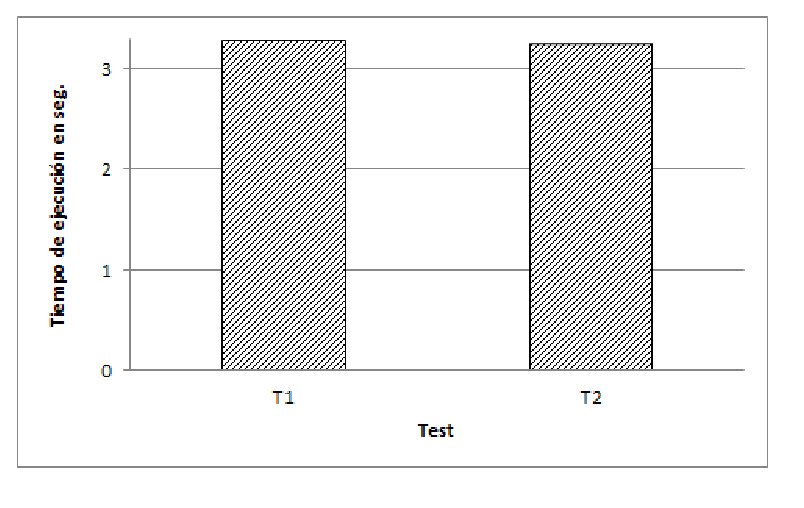
\includegraphics[width=12cm]{./images/phd/experimentation/t1-t2-tiempo}
\caption{Gráfica de Tiempo de ejecución medio con referencia $T_1$.}
\label{fig:results-graph-1}
\end{figure}

\begin{figure}[!htb]
\centering
	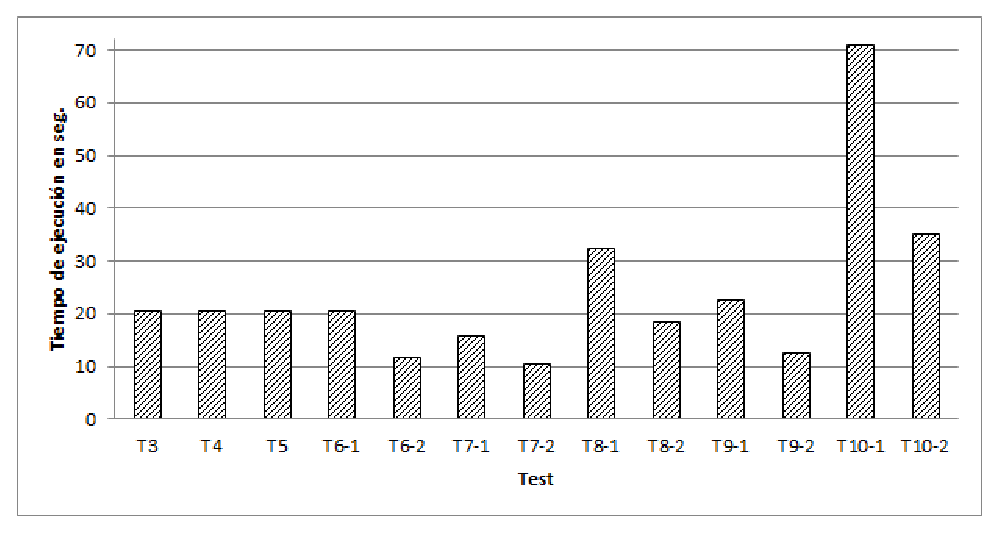
\includegraphics[width=14cm]{./images/phd/experimentation/t3-t10-tiempo}
\caption{Gráfica de Tiempo de ejecución medio con referencia $T_3$.}
\label{fig:results-graph-2}
\end{figure}

\begin{figure}[!htb]
\centering
	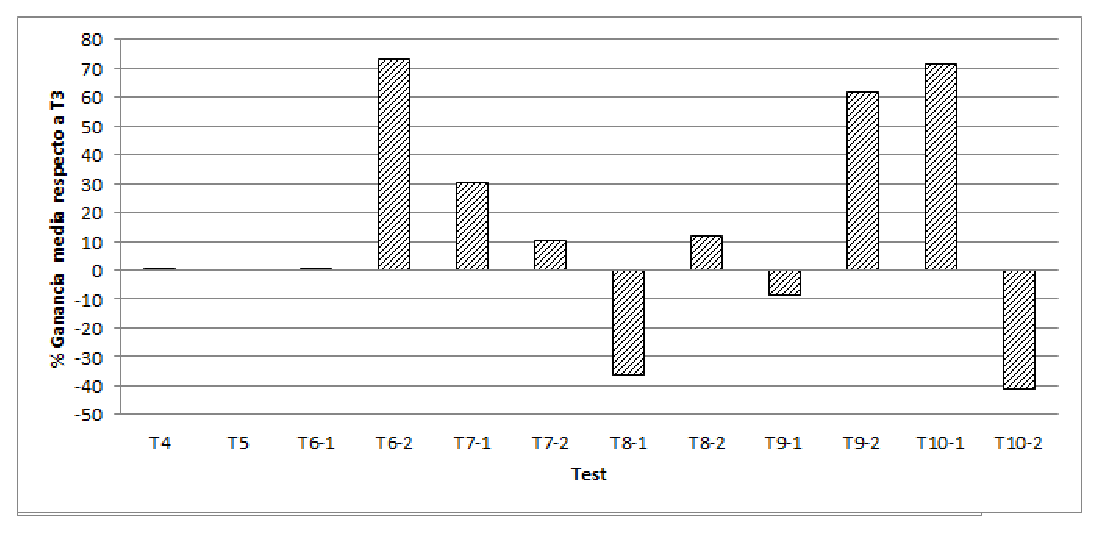
\includegraphics[width=14cm]{./images/phd/experimentation/t3-t10-ganancia}
\caption{Gráfica de Ganancia media con referencia $T_3$ en (\%).}
\label{fig:results-graph-3}
\end{figure}




Finalmente se ha realizado un \textbf{tercer experimento} empírico~\cite{Alvarez:2011:QEM:2075561.2075618} para probar la generación de consultas en SPARQL 
y el rendimiento del sistema MOLDEAS que han servido para optimizar las consultas tanto en su generación (reducción de claúsulas) como en modelo de ejecución (distribuido).


\chapter{Conclusiones y Trabajo Futuro}
La investigación, desarrollo e innovación realizado en este trabajo ha permitido en avanzar en la aplicación 
de \linkeddata y tecnologías semánticas a un dominio estratégico para la economía con son los contratos públicos. A 
continuación se listan las principales aportaciones realizadas:
\begin{itemize}
 \item Definición y aplicación de un ciclo de vida de datos enlazados abiertos al dominio 
 de la contratación pública para la mejora del proceso de publicación de información.
 \item Diseño y evaluación de la calidad de los datos de distintos proveedores.
 \item Diseño e implementación de la plataforma MOLDEAS para la agregación y enriquecimiento 
 automática de la información y datos proveniente de los anuncios de licitación pública europea teniendo 
 en cuenta la diversidad de las fuentes y cuestiones relacionadas con el multilinguismo y la multiculturalidad.
 \item Diseño e implementación de algoritmos para automáticamente realizar la búsqueda de anuncios 
 de licitación de acuerdo a un perfil de usuario.
\item Transformación a \linkeddata de más de un millón de anuncios de licitación, 9 clasificaciones estándar de productos 
y otros conjuntos de datos como organizaciones, personas y países reutilizando información y datos existentes.
\item Diseño de experimentos para el contraste de la ganancia cualitativa y cuantiativa por el uso de \lod en el dominio 
de contratación pública incluyendo el diseño de criterios de validación de los datos generados y evaluación semi-automática de los mismos.
\item Adición a la nube de datos enlazados del \dataset de clasificaciones estándar de productos~\footnote{\url{http://datahub.io/dataset/pscs-catalogue}}. Actualmente este conjunto
está siendo ampliado y reutilizado en diferentes proyectos a nivel internacional como el proyecto LOD2.
\item Difusión y participación en actividades científicas y de carácter industrial como publicación 
en revistas JCR y edición del Special Issue: ``New trends on e-Procurement applying Semantics'' en la revista JCR ``Computers in Industry''. 
Actualmente esta tesis se está utilizando en el grupo de trabajo W3C ``Open Data Spain'' en su línea sobre Contratación Pública.
\end{itemize}

Transversalmente a los objetivos específicos constratados a través de las principales aportaciones, todo el trabajo 
realizado en las definiciones teóricas, desarrollo de activos experimentales y diseño de experimentos, se ha enmarcado bajo una apuesta fiel y constante por la aplicación y uso de los estándares 
dando así acogida a la meta de ``Promover el uso de estándares y la reutilización de  información y modelos de conocimiento compartido''.

El estudio de los datos enlazados abiertos en el campo de las licitaciones públicas ha puesto de manifiesto las necesidades 
de este entorno y la necesidad de realizar una investigación profunda para impulsar la contratación pública electrónica dada 
su relevancia e impacto en la sociedad. Por ello, el enfoque basado en tecnologías semánticas y datos enlazados abiertos 
permite la culminación práctica de ciertas necesidades como la mejora de acceso y la reutilización de la información. Sin embargo, 
la conversión de un entorno tan amplio debe tomarse como una actividad iterativa, en la cual con la aplicación de buenas 
prácticas se consiga dar respuesta y solución a los inconvenientes que presenta. A continuación se detallan las conclusiones 
más relevantes.

\begin{itemize}
 \item Todos los procesos implicados en el tratamiento de datos enlazados deben asegurarse suministrando 
mecanismos para su validación con el objetivo de facilitar su reutilización posterior en condiciones 
de ausencia de incertidumbre.
  \item El uso de estándares es clave para minimizar los problemas de integración e interoperabilidad.
 \item El tratamiento de grandes cantidades de datos conlleva prestar especial atención a los algoritmos diseñados y 
a la construcción de consultas sobre los mismos.
 \item La necesidad de modelar la información y datos para su posterior reutilización en un dominio extenso debe realizarse 
con el suficiente grado de especificidad, pero teniendo presente la posibilidad de extensibilidad, por lo que es conveniente 
no realizar grandes modelos poco usables y que tan sólo el autor o autores pueden manejar. En este sentido la estrategia 
a seguir debe basarse en la generación de un marco de trabajo común y la creación sostenible y escalable de conocimiento 
con el objetivo de impulsar su reutilización.
 \item Los principios de \linkeddata y \opendata verdaderamente ayudan a favorecer la reutilización de información si siguen 
unas directrices de producción, publicación y consumo adecuadas.
 \item El maremágnum de tecnología, enfoques, algoritmos, vocabularios, conjuntos de datos, etc., dentro de la iniciativa de 
\linkeddata convierte la toma de ciertas decisiones y la adopción de soluciones en un trabajo tedioso en el cual la experiencia 
cobra una especial relevancia. 
 \item Existen tareas como la reconciliación de entidades que todavía se hayan en una etapa temprana de desarrollo.
 \item El uso de datos enlazados permite mejorar el acceso a la información facilitando una mayor expresividad en la realización 
de consultas sobre grandes conjuntos de datos.
 \item Desde el punto de vista de la gestión de la información y datos, la Web Semántica se ha convertido en una pieza clave pero 
la creación de algoritmos explotando las capacidades de un entorno mejor informado todavía no se ha impulsado convenientemente.
\item Los procesos administrativos dentro de la administración electrónica deben necesariamente aprovechar las ventajas 
de las tecnologías de información para ser más eficientes.
\item Las primeras versiones de datos enlazados abiertos liberados tendían a basar su éxito en el número de tripletas RDF. El esfuerzo se 
centra ahora en la calidad para asegurar su reutilización.
\end{itemize}

Las posibilidades de abrir nuevas líneas de investigación que tomen como semilla el trabajo realizado en este estudio son múltiples 
y se pueden abordar desde distintos puntos de vista: 1) las concernientes a la Web Semántica y \linkeddata en general y 
2) las referentes a la administración electrónica y en particular al proceso administrativo de contratación pública electrónica. Entre 
las más relevantes que ya se están llevando a cabo y surgidas tras la realización de este trabajo se encuentran:
\begin{itemize}
 \item Realización de un sistema de catalogación de vocabularios y conjuntos de datos basado en diferentes métricas.
 \item Mejora de los algoritmos de reconciliación de entidades.
 \item Adaptación y mejora de las técnicas y algoritmos basados en semántica a entornos con características de tiempo real.
 \item Realización de un sistema experto específico para la recuperación de información de anuncios de licitación teniendo en cuenta la mayor cantidad de descriptores posibles.
 \item Mejora de la capitalización del conocimiento experto en el dominio de contratación pública electrónica.
 \item Otras: procesamiento de consultas federadas de forma eficiente, búsqueda sobre fuentes de datos heterogéneas, 
 descubrimiento automático de \datasets, gestión de \datasets dinámicos, calidad de los datos, usabilidad en la interacción con datos enlazados o 
 notificación de resultados a las instituciones públicas.
\end{itemize}

Actualmente se está desarrollando la plataforma MOLDEAS2 incluyendo capacidades de búsqueda e indexado en tiempo real.

\section*{Agradecimientos}
Este trabajo ha sido desarrollado en el contexto del proyecto \textit{10ders Information Services}, proyecto de investigación
cofinanciado por el Ministerio de Industria, Turismo y Comercio dentro del plan Avanza 2 con código TSI-020100-2010-919, 
liderado por Gateway S.C.S. y desarrollado en colaboración con la empresa Exis TI y el grupo de investigación WESO de la Universidad de Oviedo. 


\chapter{Principales Aportaciones: Impacto y Difusión}

\section{Selección de artículos}
%5 y explain
%COMINDSO
\section{Selección de conferencias}
%5 y explain
%COMINDSO
\section{Participación en iniciativas internacionales}
\section{Participación en iniciativas internacionales}


%%%%%%%%%%%%%%%%%%%%%%%%%%%%%%%%%%%%%%%%%%%%%%%%%%%%%%%%%%%%%%%%%%%%%%
\backmatter


\printindex
\printglossaries


% Bibliografía
\insertbibliography
\end{document}
